\documentclass[twoside]{book}

% Packages required by doxygen
\usepackage{fixltx2e}
\usepackage{calc}
\usepackage{doxygen}
\usepackage[export]{adjustbox} % also loads graphicx
\usepackage{graphicx}
\usepackage[utf8]{inputenc}
\usepackage{makeidx}
\usepackage{multicol}
\usepackage{multirow}
\PassOptionsToPackage{warn}{textcomp}
\usepackage{textcomp}
\usepackage[nointegrals]{wasysym}
\usepackage[table]{xcolor}

% Font selection
\usepackage[T1]{fontenc}
\usepackage[scaled=.90]{helvet}
\usepackage{courier}
\usepackage{amssymb}
\usepackage{sectsty}
\renewcommand{\familydefault}{\sfdefault}
\allsectionsfont{%
  \fontseries{bc}\selectfont%
  \color{darkgray}%
}
\renewcommand{\DoxyLabelFont}{%
  \fontseries{bc}\selectfont%
  \color{darkgray}%
}
\newcommand{\+}{\discretionary{\mbox{\scriptsize$\hookleftarrow$}}{}{}}

% Page & text layout
\usepackage{geometry}
\geometry{%
  a4paper,%
  top=2.5cm,%
  bottom=2.5cm,%
  left=2.5cm,%
  right=2.5cm%
}
\tolerance=750
\hfuzz=15pt
\hbadness=750
\setlength{\emergencystretch}{15pt}
\setlength{\parindent}{0cm}
\setlength{\parskip}{3ex plus 2ex minus 2ex}
\makeatletter
\renewcommand{\paragraph}{%
  \@startsection{paragraph}{4}{0ex}{-1.0ex}{1.0ex}{%
    \normalfont\normalsize\bfseries\SS@parafont%
  }%
}
\renewcommand{\subparagraph}{%
  \@startsection{subparagraph}{5}{0ex}{-1.0ex}{1.0ex}{%
    \normalfont\normalsize\bfseries\SS@subparafont%
  }%
}
\makeatother

% Headers & footers
\usepackage{fancyhdr}
\pagestyle{fancyplain}
\fancyhead[LE]{\fancyplain{}{\bfseries\thepage}}
\fancyhead[CE]{\fancyplain{}{}}
\fancyhead[RE]{\fancyplain{}{\bfseries\leftmark}}
\fancyhead[LO]{\fancyplain{}{\bfseries\rightmark}}
\fancyhead[CO]{\fancyplain{}{}}
\fancyhead[RO]{\fancyplain{}{\bfseries\thepage}}
\fancyfoot[LE]{\fancyplain{}{}}
\fancyfoot[CE]{\fancyplain{}{}}
\fancyfoot[RE]{\fancyplain{}{\bfseries\scriptsize Generated by Doxygen }}
\fancyfoot[LO]{\fancyplain{}{\bfseries\scriptsize Generated by Doxygen }}
\fancyfoot[CO]{\fancyplain{}{}}
\fancyfoot[RO]{\fancyplain{}{}}
\renewcommand{\footrulewidth}{0.4pt}
\renewcommand{\chaptermark}[1]{%
  \markboth{#1}{}%
}
\renewcommand{\sectionmark}[1]{%
  \markright{\thesection\ #1}%
}

% Indices & bibliography
\usepackage{natbib}
\usepackage[titles]{tocloft}
\setcounter{tocdepth}{3}
\setcounter{secnumdepth}{5}
\makeindex

% Hyperlinks (required, but should be loaded last)
\usepackage{ifpdf}
\ifpdf
  \usepackage[pdftex,pagebackref=true]{hyperref}
\else
  \usepackage[ps2pdf,pagebackref=true]{hyperref}
\fi
\hypersetup{%
  colorlinks=true,%
  linkcolor=blue,%
  citecolor=blue,%
  unicode%
}

% Custom commands
\newcommand{\clearemptydoublepage}{%
  \newpage{\pagestyle{empty}\cleardoublepage}%
}

\usepackage{caption}
\captionsetup{labelsep=space,justification=centering,font={bf},singlelinecheck=off,skip=4pt,position=top}

%===== C O N T E N T S =====

\begin{document}

% Titlepage & ToC
\hypersetup{pageanchor=false,
             bookmarksnumbered=true,
             pdfencoding=unicode
            }
\pagenumbering{alph}
\begin{titlepage}
\vspace*{7cm}
\begin{center}%
{\Large Bomber\+Dude \\[1ex]\large 1.\+000000000001 }\\
\vspace*{1cm}
{\large Generated by Doxygen 1.8.12}\\
\end{center}
\end{titlepage}
\clearemptydoublepage
\pagenumbering{roman}
\tableofcontents
\clearemptydoublepage
\pagenumbering{arabic}
\hypersetup{pageanchor=true}

%--- Begin generated contents ---
\chapter{Namespace Index}
\section{Namespace List}
Here is a list of all namespaces with brief descriptions\+:\begin{DoxyCompactList}
\item\contentsline{section}{\hyperlink{namespaceerror}{error} }{\pageref{namespaceerror}}{}
\end{DoxyCompactList}

\chapter{Hierarchical Index}
\section{Class Hierarchy}
This inheritance list is sorted roughly, but not completely, alphabetically\+:\begin{DoxyCompactList}
\item \contentsline{section}{Application}{\pageref{class_application}}{}
\item \contentsline{section}{Bomb}{\pageref{class_bomb}}{}
\item \contentsline{section}{Bomb\+Packet}{\pageref{struct_bomb_packet}}{}
\item \contentsline{section}{Debug\+UI}{\pageref{class_debug_u_i}}{}
\item \contentsline{section}{Player\+Character}{\pageref{class_player_character}}{}
\begin{DoxyCompactList}
\item \contentsline{section}{Networked\+Character}{\pageref{class_networked_character}}{}
\end{DoxyCompactList}
\item \contentsline{section}{Player\+Update\+Packet}{\pageref{struct_player_update_packet}}{}
\item \contentsline{section}{Timed\+Message}{\pageref{struct_timed_message}}{}
\item \contentsline{section}{Time\+Position\+Struct}{\pageref{struct_time_position_struct}}{}
\item \contentsline{section}{Welcome\+Packet}{\pageref{struct_welcome_packet}}{}
\item \contentsline{section}{Welcome\+Packet\+Reply}{\pageref{struct_welcome_packet_reply}}{}
\end{DoxyCompactList}

\chapter{Class Index}
\section{Class List}
Here are the classes, structs, unions and interfaces with brief descriptions\+:\begin{DoxyCompactList}
\item\contentsline{section}{\hyperlink{class_application}{Application} }{\pageref{class_application}}{}
\item\contentsline{section}{\hyperlink{class_bomb}{Bomb} }{\pageref{class_bomb}}{}
\item\contentsline{section}{\hyperlink{struct_bomb_packet}{Bomb\+Packet} }{\pageref{struct_bomb_packet}}{}
\item\contentsline{section}{\hyperlink{class_debug_u_i}{Debug\+UI} }{\pageref{class_debug_u_i}}{}
\item\contentsline{section}{\hyperlink{class_networked_character}{Networked\+Character} }{\pageref{class_networked_character}}{}
\item\contentsline{section}{\hyperlink{class_player_character}{Player\+Character} }{\pageref{class_player_character}}{}
\item\contentsline{section}{\hyperlink{struct_player_update_packet}{Player\+Update\+Packet} }{\pageref{struct_player_update_packet}}{}
\item\contentsline{section}{\hyperlink{struct_timed_message}{Timed\+Message} }{\pageref{struct_timed_message}}{}
\item\contentsline{section}{\hyperlink{struct_time_position_struct}{Time\+Position\+Struct} }{\pageref{struct_time_position_struct}}{}
\item\contentsline{section}{\hyperlink{struct_welcome_packet}{Welcome\+Packet} }{\pageref{struct_welcome_packet}}{}
\item\contentsline{section}{\hyperlink{struct_welcome_packet_reply}{Welcome\+Packet\+Reply} }{\pageref{struct_welcome_packet_reply}}{}
\end{DoxyCompactList}

\chapter{File Index}
\section{File List}
Here is a list of all files with brief descriptions\+:\begin{DoxyCompactList}
\item\contentsline{section}{E\+:/\+Coding/\+S\+F\+M\+L\+\_\+\+Networked\+Game/\+Networking\+Coursework/\hyperlink{_application_8cpp}{Application.\+cpp} }{\pageref{_application_8cpp}}{}
\item\contentsline{section}{E\+:/\+Coding/\+S\+F\+M\+L\+\_\+\+Networked\+Game/\+Networking\+Coursework/\hyperlink{_application_8h}{Application.\+h} }{\pageref{_application_8h}}{}
\item\contentsline{section}{E\+:/\+Coding/\+S\+F\+M\+L\+\_\+\+Networked\+Game/\+Networking\+Coursework/\hyperlink{_bomb_8cpp}{Bomb.\+cpp} }{\pageref{_bomb_8cpp}}{}
\item\contentsline{section}{E\+:/\+Coding/\+S\+F\+M\+L\+\_\+\+Networked\+Game/\+Networking\+Coursework/\hyperlink{_bomb_8h}{Bomb.\+h} }{\pageref{_bomb_8h}}{}
\item\contentsline{section}{E\+:/\+Coding/\+S\+F\+M\+L\+\_\+\+Networked\+Game/\+Networking\+Coursework/\hyperlink{_debug_u_i_8cpp}{Debug\+U\+I.\+cpp} }{\pageref{_debug_u_i_8cpp}}{}
\item\contentsline{section}{E\+:/\+Coding/\+S\+F\+M\+L\+\_\+\+Networked\+Game/\+Networking\+Coursework/\hyperlink{_debug_u_i_8h}{Debug\+U\+I.\+h} }{\pageref{_debug_u_i_8h}}{}
\item\contentsline{section}{E\+:/\+Coding/\+S\+F\+M\+L\+\_\+\+Networked\+Game/\+Networking\+Coursework/\hyperlink{_error_system_8cpp}{Error\+System.\+cpp} }{\pageref{_error_system_8cpp}}{}
\item\contentsline{section}{E\+:/\+Coding/\+S\+F\+M\+L\+\_\+\+Networked\+Game/\+Networking\+Coursework/\hyperlink{_error_system_8h}{Error\+System.\+h} }{\pageref{_error_system_8h}}{}
\item\contentsline{section}{E\+:/\+Coding/\+S\+F\+M\+L\+\_\+\+Networked\+Game/\+Networking\+Coursework/\hyperlink{_networked_character_8cpp}{Networked\+Character.\+cpp} }{\pageref{_networked_character_8cpp}}{}
\item\contentsline{section}{E\+:/\+Coding/\+S\+F\+M\+L\+\_\+\+Networked\+Game/\+Networking\+Coursework/\hyperlink{_networked_character_8h}{Networked\+Character.\+h} }{\pageref{_networked_character_8h}}{}
\item\contentsline{section}{E\+:/\+Coding/\+S\+F\+M\+L\+\_\+\+Networked\+Game/\+Networking\+Coursework/\hyperlink{_player_character_8cpp}{Player\+Character.\+cpp} }{\pageref{_player_character_8cpp}}{}
\item\contentsline{section}{E\+:/\+Coding/\+S\+F\+M\+L\+\_\+\+Networked\+Game/\+Networking\+Coursework/\hyperlink{_player_character_8h}{Player\+Character.\+h} }{\pageref{_player_character_8h}}{}
\item\contentsline{section}{E\+:/\+Coding/\+S\+F\+M\+L\+\_\+\+Networked\+Game/\+Networking\+Coursework/\hyperlink{_source_8cpp}{Source.\+cpp} }{\pageref{_source_8cpp}}{}
\end{DoxyCompactList}

\chapter{Namespace Documentation}
\hypertarget{namespaceerror}{}\section{error Namespace Reference}
\label{namespaceerror}\index{error@{error}}
\subsection*{Functions}
\begin{DoxyCompactItemize}
\item 
void \hyperlink{namespaceerror_a019f42947a3ea3414560875df66d5eb5}{Value\+Error} (std\+::string id, std\+::string message, float value, bool destroy\+\_\+window=true)
\item 
void \hyperlink{namespaceerror_a7d5d0c6be08af9155409c2f1c900dbb1}{Value\+Error} (std\+::string id, std\+::string message, int value, bool destroy\+\_\+window=true)
\item 
void \hyperlink{namespaceerror_a6d9707ac0b5ce39b0bcd7b37862a47b4}{Error\+Message} (std\+::string message, bool destroy\+\_\+window=true)
\item 
void \hyperlink{namespaceerror_a66d4ae4163a05f4ee9b28831c6c8118a}{String\+Error} (std\+::string id, std\+::string message, bool destroy\+\_\+window=true)
\end{DoxyCompactItemize}


\subsection{Detailed Description}
The Windows Based Error System

For quickly showing errors incase of out of range values etc allows for custom prompts and ID sortin 

\subsection{Function Documentation}
\hypertarget{namespaceerror_a6d9707ac0b5ce39b0bcd7b37862a47b4}{}\label{namespaceerror_a6d9707ac0b5ce39b0bcd7b37862a47b4} 
\index{error@{error}!Error\+Message@{Error\+Message}}
\index{Error\+Message@{Error\+Message}!error@{error}}
\subsubsection{\texorpdfstring{Error\+Message()}{ErrorMessage()}}
{\footnotesize\ttfamily void error\+::\+Error\+Message (\begin{DoxyParamCaption}\item[{std\+::string}]{message,  }\item[{bool}]{destroy\+\_\+window = {\ttfamily true} }\end{DoxyParamCaption})}

\hypertarget{namespaceerror_a66d4ae4163a05f4ee9b28831c6c8118a}{}\label{namespaceerror_a66d4ae4163a05f4ee9b28831c6c8118a} 
\index{error@{error}!String\+Error@{String\+Error}}
\index{String\+Error@{String\+Error}!error@{error}}
\subsubsection{\texorpdfstring{String\+Error()}{StringError()}}
{\footnotesize\ttfamily void error\+::\+String\+Error (\begin{DoxyParamCaption}\item[{std\+::string}]{id,  }\item[{std\+::string}]{message,  }\item[{bool}]{destroy\+\_\+window = {\ttfamily true} }\end{DoxyParamCaption})}

\hypertarget{namespaceerror_a019f42947a3ea3414560875df66d5eb5}{}\label{namespaceerror_a019f42947a3ea3414560875df66d5eb5} 
\index{error@{error}!Value\+Error@{Value\+Error}}
\index{Value\+Error@{Value\+Error}!error@{error}}
\subsubsection{\texorpdfstring{Value\+Error()}{ValueError()}\hspace{0.1cm}{\footnotesize\ttfamily [1/2]}}
{\footnotesize\ttfamily void error\+::\+Value\+Error (\begin{DoxyParamCaption}\item[{std\+::string}]{id,  }\item[{std\+::string}]{message,  }\item[{float}]{value,  }\item[{bool}]{destroy\+\_\+window = {\ttfamily true} }\end{DoxyParamCaption})}

\hypertarget{namespaceerror_a7d5d0c6be08af9155409c2f1c900dbb1}{}\label{namespaceerror_a7d5d0c6be08af9155409c2f1c900dbb1} 
\index{error@{error}!Value\+Error@{Value\+Error}}
\index{Value\+Error@{Value\+Error}!error@{error}}
\subsubsection{\texorpdfstring{Value\+Error()}{ValueError()}\hspace{0.1cm}{\footnotesize\ttfamily [2/2]}}
{\footnotesize\ttfamily void error\+::\+Value\+Error (\begin{DoxyParamCaption}\item[{std\+::string}]{id,  }\item[{std\+::string}]{message,  }\item[{int}]{value,  }\item[{bool}]{destroy\+\_\+window = {\ttfamily true} }\end{DoxyParamCaption})}


\chapter{Class Documentation}
\hypertarget{class_application}{}\section{Application Class Reference}
\label{class_application}\index{Application@{Application}}


{\ttfamily \#include $<$Application.\+h$>$}

\subsection*{Public Member Functions}
\begin{DoxyCompactItemize}
\item 
\hyperlink{class_application_afa8cc05ce6b6092be5ecdfdae44e05f8}{Application} ()
\item 
\hyperlink{class_application_a748bca84fefb9c12661cfaa2f623748d}{$\sim$\+Application} ()
\item 
void \hyperlink{class_application_a2e40123b025f8cab8fee0120792f670a}{Init} (sf\+::\+Render\+Window $\ast$Window, int Screen\+Width, int Screen\+Height)
\item 
void \hyperlink{class_application_a28c5c9dba1b7a8ca51b54b6e624c22b6}{Update} (float dt)
\item 
void \hyperlink{class_application_a6f40ffdb97f3a938ae19ea4eae4882ed}{Render} ()
\end{DoxyCompactItemize}


\subsection{Detailed Description}
The \hyperlink{class_application}{Application} Class

This is the main Game Loop controller Thats and an initialisation an Update and a Render Function which will be run from the main.\+ccp 

\subsection{Constructor \& Destructor Documentation}
\hypertarget{class_application_afa8cc05ce6b6092be5ecdfdae44e05f8}{}\label{class_application_afa8cc05ce6b6092be5ecdfdae44e05f8} 
\index{Application@{Application}!Application@{Application}}
\index{Application@{Application}!Application@{Application}}
\subsubsection{\texorpdfstring{Application()}{Application()}}
{\footnotesize\ttfamily Application\+::\+Application (\begin{DoxyParamCaption}{ }\end{DoxyParamCaption})}

\hypertarget{class_application_a748bca84fefb9c12661cfaa2f623748d}{}\label{class_application_a748bca84fefb9c12661cfaa2f623748d} 
\index{Application@{Application}!````~Application@{$\sim$\+Application}}
\index{````~Application@{$\sim$\+Application}!Application@{Application}}
\subsubsection{\texorpdfstring{$\sim$\+Application()}{~Application()}}
{\footnotesize\ttfamily Application\+::$\sim$\+Application (\begin{DoxyParamCaption}{ }\end{DoxyParamCaption})}



\subsection{Member Function Documentation}
\hypertarget{class_application_a2e40123b025f8cab8fee0120792f670a}{}\label{class_application_a2e40123b025f8cab8fee0120792f670a} 
\index{Application@{Application}!Init@{Init}}
\index{Init@{Init}!Application@{Application}}
\subsubsection{\texorpdfstring{Init()}{Init()}}
{\footnotesize\ttfamily void Application\+::\+Init (\begin{DoxyParamCaption}\item[{sf\+::\+Render\+Window $\ast$}]{Window,  }\item[{int}]{Screen\+Width,  }\item[{int}]{Screen\+Height }\end{DoxyParamCaption})}

The Intialiser function Will initialse all variables and set up the player/server/client


\begin{DoxyParams}{Parameters}
{\em Render\+Window} & pointer to the created S\+F\+ML window \\
\hline
{\em Screen\+Width} & the set screen width \\
\hline
{\em Screen\+Height} & the set screen height \\
\hline
\end{DoxyParams}
\hypertarget{class_application_a6f40ffdb97f3a938ae19ea4eae4882ed}{}\label{class_application_a6f40ffdb97f3a938ae19ea4eae4882ed} 
\index{Application@{Application}!Render@{Render}}
\index{Render@{Render}!Application@{Application}}
\subsubsection{\texorpdfstring{Render()}{Render()}}
{\footnotesize\ttfamily void Application\+::\+Render (\begin{DoxyParamCaption}{ }\end{DoxyParamCaption})}

Render all objects to the S\+F\+ML window \hypertarget{class_application_a28c5c9dba1b7a8ca51b54b6e624c22b6}{}\label{class_application_a28c5c9dba1b7a8ca51b54b6e624c22b6} 
\index{Application@{Application}!Update@{Update}}
\index{Update@{Update}!Application@{Application}}
\subsubsection{\texorpdfstring{Update()}{Update()}}
{\footnotesize\ttfamily void Application\+::\+Update (\begin{DoxyParamCaption}\item[{float}]{dt }\end{DoxyParamCaption})}

Update the main game loop


\begin{DoxyParams}{Parameters}
{\em delta} & time \\
\hline
\end{DoxyParams}


The documentation for this class was generated from the following files\+:\begin{DoxyCompactItemize}
\item 
E\+:/\+Coding/\+S\+F\+M\+L\+\_\+\+Networked\+Game/\+Networking\+Coursework/\hyperlink{_application_8h}{Application.\+h}\item 
E\+:/\+Coding/\+S\+F\+M\+L\+\_\+\+Networked\+Game/\+Networking\+Coursework/\hyperlink{_application_8cpp}{Application.\+cpp}\end{DoxyCompactItemize}

\hypertarget{class_bomb}{}\section{Bomb Class Reference}
\label{class_bomb}\index{Bomb@{Bomb}}


{\ttfamily \#include $<$Bomb.\+h$>$}

\subsection*{Public Member Functions}
\begin{DoxyCompactItemize}
\item 
\hyperlink{class_bomb_a70f8313ed21a19605a1ee6f65b6eaf18}{Bomb} (sf\+::\+Vector2f Position, float Time\+To\+Explode)
\item 
\hyperlink{class_bomb_acbb47327cfb2fa429887774ef3597965}{$\sim$\+Bomb} ()
\item 
void \hyperlink{class_bomb_a824b48a1cabce718db5b9b0c84452a35}{Update} (float dt, float Current\+Time)
\item 
void \hyperlink{class_bomb_af676fc06d6ede72f26fe4d7602e41ffa}{Render} (sf\+::\+Render\+Window $\ast$Window)
\item 
bool \hyperlink{class_bomb_a787ba65ab16bdcb5ff622ff2395e743f}{Is\+Exploded} ()
\end{DoxyCompactItemize}


\subsection{Detailed Description}
The \hyperlink{class_bomb}{Bomb} class will Display bombs and the screen and blow up after a given time 

\subsection{Constructor \& Destructor Documentation}
\hypertarget{class_bomb_a70f8313ed21a19605a1ee6f65b6eaf18}{}\label{class_bomb_a70f8313ed21a19605a1ee6f65b6eaf18} 
\index{Bomb@{Bomb}!Bomb@{Bomb}}
\index{Bomb@{Bomb}!Bomb@{Bomb}}
\subsubsection{\texorpdfstring{Bomb()}{Bomb()}}
{\footnotesize\ttfamily Bomb\+::\+Bomb (\begin{DoxyParamCaption}\item[{sf\+::\+Vector2f}]{Position,  }\item[{float}]{Time\+To\+Explode }\end{DoxyParamCaption})}

The \hyperlink{class_bomb}{Bomb} Constructor


\begin{DoxyParams}{Parameters}
{\em Positon} & of the bomb to be placed \\
\hline
{\em The} & Server time in which it should explode \\
\hline
\end{DoxyParams}
\hypertarget{class_bomb_acbb47327cfb2fa429887774ef3597965}{}\label{class_bomb_acbb47327cfb2fa429887774ef3597965} 
\index{Bomb@{Bomb}!````~Bomb@{$\sim$\+Bomb}}
\index{````~Bomb@{$\sim$\+Bomb}!Bomb@{Bomb}}
\subsubsection{\texorpdfstring{$\sim$\+Bomb()}{~Bomb()}}
{\footnotesize\ttfamily Bomb\+::$\sim$\+Bomb (\begin{DoxyParamCaption}{ }\end{DoxyParamCaption})}



\subsection{Member Function Documentation}
\hypertarget{class_bomb_a787ba65ab16bdcb5ff622ff2395e743f}{}\label{class_bomb_a787ba65ab16bdcb5ff622ff2395e743f} 
\index{Bomb@{Bomb}!Is\+Exploded@{Is\+Exploded}}
\index{Is\+Exploded@{Is\+Exploded}!Bomb@{Bomb}}
\subsubsection{\texorpdfstring{Is\+Exploded()}{IsExploded()}}
{\footnotesize\ttfamily bool Bomb\+::\+Is\+Exploded (\begin{DoxyParamCaption}{ }\end{DoxyParamCaption})\hspace{0.3cm}{\ttfamily [inline]}}

Returns if the bomb has exploded or not \begin{DoxyReturn}{Returns}
true if bomb exploded 
\end{DoxyReturn}
\hypertarget{class_bomb_af676fc06d6ede72f26fe4d7602e41ffa}{}\label{class_bomb_af676fc06d6ede72f26fe4d7602e41ffa} 
\index{Bomb@{Bomb}!Render@{Render}}
\index{Render@{Render}!Bomb@{Bomb}}
\subsubsection{\texorpdfstring{Render()}{Render()}}
{\footnotesize\ttfamily void Bomb\+::\+Render (\begin{DoxyParamCaption}\item[{sf\+::\+Render\+Window $\ast$}]{Window }\end{DoxyParamCaption})}

Render in the Selected Window


\begin{DoxyParams}{Parameters}
{\em The} & S\+F\+ML Window pointer \\
\hline
\end{DoxyParams}
\hypertarget{class_bomb_a824b48a1cabce718db5b9b0c84452a35}{}\label{class_bomb_a824b48a1cabce718db5b9b0c84452a35} 
\index{Bomb@{Bomb}!Update@{Update}}
\index{Update@{Update}!Bomb@{Bomb}}
\subsubsection{\texorpdfstring{Update()}{Update()}}
{\footnotesize\ttfamily void Bomb\+::\+Update (\begin{DoxyParamCaption}\item[{float}]{dt,  }\item[{float}]{Current\+Time }\end{DoxyParamCaption})}

Update the bombs -\/ Checks if the should explode against the current time


\begin{DoxyParams}{Parameters}
{\em Delta} & time \\
\hline
{\em Current} & Game Time \\
\hline
\end{DoxyParams}


The documentation for this class was generated from the following files\+:\begin{DoxyCompactItemize}
\item 
E\+:/\+Coding/\+S\+F\+M\+L\+\_\+\+Networked\+Game/\+Networking\+Coursework/\hyperlink{_bomb_8h}{Bomb.\+h}\item 
E\+:/\+Coding/\+S\+F\+M\+L\+\_\+\+Networked\+Game/\+Networking\+Coursework/\hyperlink{_bomb_8cpp}{Bomb.\+cpp}\end{DoxyCompactItemize}

\hypertarget{struct_bomb_packet}{}\section{Bomb\+Packet Struct Reference}
\label{struct_bomb_packet}\index{Bomb\+Packet@{Bomb\+Packet}}


{\ttfamily \#include $<$Application.\+h$>$}

\subsection*{Public Attributes}
\begin{DoxyCompactItemize}
\item 
float \hyperlink{struct_bomb_packet_ae2c558c55820bf97e954370743222224}{Xpos}
\item 
float \hyperlink{struct_bomb_packet_a5279e358c68ee4506035cb2855352955}{Ypos}
\item 
float \hyperlink{struct_bomb_packet_a7d44fc787b6cb299267bb2a1a5a61dd2}{Time\+To\+Explode}
\end{DoxyCompactItemize}


\subsection{Detailed Description}
\hyperlink{class_bomb}{Bomb} Packet

Has the position of the bomb and the time it will explode 

\subsection{Member Data Documentation}
\hypertarget{struct_bomb_packet_a7d44fc787b6cb299267bb2a1a5a61dd2}{}\label{struct_bomb_packet_a7d44fc787b6cb299267bb2a1a5a61dd2} 
\index{Bomb\+Packet@{Bomb\+Packet}!Time\+To\+Explode@{Time\+To\+Explode}}
\index{Time\+To\+Explode@{Time\+To\+Explode}!Bomb\+Packet@{Bomb\+Packet}}
\subsubsection{\texorpdfstring{Time\+To\+Explode}{TimeToExplode}}
{\footnotesize\ttfamily float Bomb\+Packet\+::\+Time\+To\+Explode}

\hypertarget{struct_bomb_packet_ae2c558c55820bf97e954370743222224}{}\label{struct_bomb_packet_ae2c558c55820bf97e954370743222224} 
\index{Bomb\+Packet@{Bomb\+Packet}!Xpos@{Xpos}}
\index{Xpos@{Xpos}!Bomb\+Packet@{Bomb\+Packet}}
\subsubsection{\texorpdfstring{Xpos}{Xpos}}
{\footnotesize\ttfamily float Bomb\+Packet\+::\+Xpos}

\hypertarget{struct_bomb_packet_a5279e358c68ee4506035cb2855352955}{}\label{struct_bomb_packet_a5279e358c68ee4506035cb2855352955} 
\index{Bomb\+Packet@{Bomb\+Packet}!Ypos@{Ypos}}
\index{Ypos@{Ypos}!Bomb\+Packet@{Bomb\+Packet}}
\subsubsection{\texorpdfstring{Ypos}{Ypos}}
{\footnotesize\ttfamily float Bomb\+Packet\+::\+Ypos}



The documentation for this struct was generated from the following file\+:\begin{DoxyCompactItemize}
\item 
E\+:/\+Coding/\+S\+F\+M\+L\+\_\+\+Networked\+Game/\+Networking\+Coursework/\hyperlink{_application_8h}{Application.\+h}\end{DoxyCompactItemize}

\hypertarget{class_debug_u_i}{}\section{Debug\+UI Class Reference}
\label{class_debug_u_i}\index{Debug\+UI@{Debug\+UI}}


{\ttfamily \#include $<$Debug\+U\+I.\+h$>$}

\subsection*{Public Member Functions}
\begin{DoxyCompactItemize}
\item 
\hyperlink{class_debug_u_i_a4b3d4e2cb69eff1e1dd7c9fa4070601a}{Debug\+UI} ()
\item 
\hyperlink{class_debug_u_i_a9c08c8a56117976e4b3a6873248f1ced}{$\sim$\+Debug\+UI} ()
\item 
void \hyperlink{class_debug_u_i_aeff0255f8d3c420a10ed04e665555774}{Init} (std\+::string Font\+File\+Name, int Message\+Box\+PosX, int Message\+Box\+PosY)
\item 
void \hyperlink{class_debug_u_i_afdb947e24f6aef1fdbbed54ee275cd46}{Render} (sf\+::\+Render\+Window $\ast$Window)
\item 
void \hyperlink{class_debug_u_i_a9cd779b785ef78f23ad8fb0f9e5e469a}{Update} ()
\item 
sf\+::\+Text $\ast$ \hyperlink{class_debug_u_i_a16964cf8ac1665e9dda3e86cc84f0483}{Add\+To\+Debug\+Screen} (std\+::string Initial\+String, int X\+Pos, int Y\+Pos, \hyperlink{_debug_u_i_8h_a508b2d1c58a6b1f2f8d1afdab60a289d}{Debug\+Colour} Colour=\hyperlink{_debug_u_i_8h_a508b2d1c58a6b1f2f8d1afdab60a289da3ed70705a90c9992072dc9362e041515}{k\+White\+Colour})
\item 
void \hyperlink{class_debug_u_i_a8bdf11a44f6308e6ac7a3fb9e9c15cc6}{Add\+Message} (std\+::string Message, \hyperlink{_debug_u_i_8h_a508b2d1c58a6b1f2f8d1afdab60a289d}{Debug\+Colour} Colour=\hyperlink{_debug_u_i_8h_a508b2d1c58a6b1f2f8d1afdab60a289da3ed70705a90c9992072dc9362e041515}{k\+White\+Colour}, float Time\+Delay=\hyperlink{_debug_u_i_8h_acac3d24a4253633d5c6fc707dff813ca}{M\+E\+S\+S\+A\+G\+E\+\_\+\+D\+E\+L\+E\+T\+E\+\_\+\+D\+E\+L\+AY})
\end{DoxyCompactItemize}


\subsection{Detailed Description}
T\+HE D\+E\+B\+UG C\+L\+A\+SS

The Debug class was created to help display Text on the screen Rather than creating alot of text objects and worrying about Wheter they should render or not The debug class will manage this for us. Add Text to the debug screen should be done in the init functions (W\+A\+R\+N\+I\+NG\+: N\+E\+V\+ER IN W\+H\+I\+LE L\+O\+OP) It will return a pointer to a text object that you can manage This is pushed on to a list of Text objects that the debug class will render

Messages will be strings that appear on screen and delete after a small moment of time -\/ can be added in main game loop 

\subsection{Constructor \& Destructor Documentation}
\hypertarget{class_debug_u_i_a4b3d4e2cb69eff1e1dd7c9fa4070601a}{}\label{class_debug_u_i_a4b3d4e2cb69eff1e1dd7c9fa4070601a} 
\index{Debug\+UI@{Debug\+UI}!Debug\+UI@{Debug\+UI}}
\index{Debug\+UI@{Debug\+UI}!Debug\+UI@{Debug\+UI}}
\subsubsection{\texorpdfstring{Debug\+U\+I()}{DebugUI()}}
{\footnotesize\ttfamily Debug\+U\+I\+::\+Debug\+UI (\begin{DoxyParamCaption}{ }\end{DoxyParamCaption})}

\hypertarget{class_debug_u_i_a9c08c8a56117976e4b3a6873248f1ced}{}\label{class_debug_u_i_a9c08c8a56117976e4b3a6873248f1ced} 
\index{Debug\+UI@{Debug\+UI}!````~Debug\+UI@{$\sim$\+Debug\+UI}}
\index{````~Debug\+UI@{$\sim$\+Debug\+UI}!Debug\+UI@{Debug\+UI}}
\subsubsection{\texorpdfstring{$\sim$\+Debug\+U\+I()}{~DebugUI()}}
{\footnotesize\ttfamily Debug\+U\+I\+::$\sim$\+Debug\+UI (\begin{DoxyParamCaption}{ }\end{DoxyParamCaption})}



\subsection{Member Function Documentation}
\hypertarget{class_debug_u_i_a8bdf11a44f6308e6ac7a3fb9e9c15cc6}{}\label{class_debug_u_i_a8bdf11a44f6308e6ac7a3fb9e9c15cc6} 
\index{Debug\+UI@{Debug\+UI}!Add\+Message@{Add\+Message}}
\index{Add\+Message@{Add\+Message}!Debug\+UI@{Debug\+UI}}
\subsubsection{\texorpdfstring{Add\+Message()}{AddMessage()}}
{\footnotesize\ttfamily void Debug\+U\+I\+::\+Add\+Message (\begin{DoxyParamCaption}\item[{std\+::string}]{Message,  }\item[{\hyperlink{_debug_u_i_8h_a508b2d1c58a6b1f2f8d1afdab60a289d}{Debug\+Colour}}]{Colour = {\ttfamily \hyperlink{_debug_u_i_8h_a508b2d1c58a6b1f2f8d1afdab60a289da3ed70705a90c9992072dc9362e041515}{k\+White\+Colour}},  }\item[{float}]{Time\+Delay = {\ttfamily \hyperlink{_debug_u_i_8h_acac3d24a4253633d5c6fc707dff813ca}{M\+E\+S\+S\+A\+G\+E\+\_\+\+D\+E\+L\+E\+T\+E\+\_\+\+D\+E\+L\+AY}} }\end{DoxyParamCaption})}

Add message Will add a once off message to be displayed in the message box


\begin{DoxyParams}{Parameters}
{\em The} & message to be displayd \\
\hline
{\em The} & Colour \\
\hline
{\em the} & time the message will stay on the screen -\/ Set to default if not overriden \\
\hline
\end{DoxyParams}
\hypertarget{class_debug_u_i_a16964cf8ac1665e9dda3e86cc84f0483}{}\label{class_debug_u_i_a16964cf8ac1665e9dda3e86cc84f0483} 
\index{Debug\+UI@{Debug\+UI}!Add\+To\+Debug\+Screen@{Add\+To\+Debug\+Screen}}
\index{Add\+To\+Debug\+Screen@{Add\+To\+Debug\+Screen}!Debug\+UI@{Debug\+UI}}
\subsubsection{\texorpdfstring{Add\+To\+Debug\+Screen()}{AddToDebugScreen()}}
{\footnotesize\ttfamily sf\+::\+Text $\ast$ Debug\+U\+I\+::\+Add\+To\+Debug\+Screen (\begin{DoxyParamCaption}\item[{std\+::string}]{Initial\+String,  }\item[{int}]{X\+Pos,  }\item[{int}]{Y\+Pos,  }\item[{\hyperlink{_debug_u_i_8h_a508b2d1c58a6b1f2f8d1afdab60a289d}{Debug\+Colour}}]{Colour = {\ttfamily \hyperlink{_debug_u_i_8h_a508b2d1c58a6b1f2f8d1afdab60a289da3ed70705a90c9992072dc9362e041515}{k\+White\+Colour}} }\end{DoxyParamCaption})}

Add To Debug Screen is an initialiser funciton that will display text on the screen. It will return a pointer to a Text object that can be update to change what is said on the display in run time.


\begin{DoxyParams}{Parameters}
{\em The} & Starting String \\
\hline
{\em the} & x positon of the text display \\
\hline
{\em the} & y positon of the text display \\
\hline
{\em the} & Colour of the Text \\
\hline
\end{DoxyParams}
\hypertarget{class_debug_u_i_aeff0255f8d3c420a10ed04e665555774}{}\label{class_debug_u_i_aeff0255f8d3c420a10ed04e665555774} 
\index{Debug\+UI@{Debug\+UI}!Init@{Init}}
\index{Init@{Init}!Debug\+UI@{Debug\+UI}}
\subsubsection{\texorpdfstring{Init()}{Init()}}
{\footnotesize\ttfamily void Debug\+U\+I\+::\+Init (\begin{DoxyParamCaption}\item[{std\+::string}]{Font\+File\+Name,  }\item[{int}]{Message\+Box\+PosX,  }\item[{int}]{Message\+Box\+PosY }\end{DoxyParamCaption})}

Initialsier


\begin{DoxyParams}{Parameters}
{\em Font} & File name for the font to be used \\
\hline
{\em the} & positon of the message box x/y \\
\hline
\end{DoxyParams}
\hypertarget{class_debug_u_i_afdb947e24f6aef1fdbbed54ee275cd46}{}\label{class_debug_u_i_afdb947e24f6aef1fdbbed54ee275cd46} 
\index{Debug\+UI@{Debug\+UI}!Render@{Render}}
\index{Render@{Render}!Debug\+UI@{Debug\+UI}}
\subsubsection{\texorpdfstring{Render()}{Render()}}
{\footnotesize\ttfamily void Debug\+U\+I\+::\+Render (\begin{DoxyParamCaption}\item[{sf\+::\+Render\+Window $\ast$}]{Window }\end{DoxyParamCaption})}

Render funciton


\begin{DoxyParams}{Parameters}
{\em Pointer} & to the S\+F\+ML window \\
\hline
\end{DoxyParams}
\hypertarget{class_debug_u_i_a9cd779b785ef78f23ad8fb0f9e5e469a}{}\label{class_debug_u_i_a9cd779b785ef78f23ad8fb0f9e5e469a} 
\index{Debug\+UI@{Debug\+UI}!Update@{Update}}
\index{Update@{Update}!Debug\+UI@{Debug\+UI}}
\subsubsection{\texorpdfstring{Update()}{Update()}}
{\footnotesize\ttfamily void Debug\+U\+I\+::\+Update (\begin{DoxyParamCaption}{ }\end{DoxyParamCaption})}



The documentation for this class was generated from the following files\+:\begin{DoxyCompactItemize}
\item 
E\+:/\+Coding/\+S\+F\+M\+L\+\_\+\+Networked\+Game/\+Networking\+Coursework/\hyperlink{_debug_u_i_8h}{Debug\+U\+I.\+h}\item 
E\+:/\+Coding/\+S\+F\+M\+L\+\_\+\+Networked\+Game/\+Networking\+Coursework/\hyperlink{_debug_u_i_8cpp}{Debug\+U\+I.\+cpp}\end{DoxyCompactItemize}

\hypertarget{class_networked_character}{}\section{Networked\+Character Class Reference}
\label{class_networked_character}\index{Networked\+Character@{Networked\+Character}}


{\ttfamily \#include $<$Networked\+Character.\+h$>$}

Inheritance diagram for Networked\+Character\+:\begin{figure}[H]
\begin{center}
\leavevmode
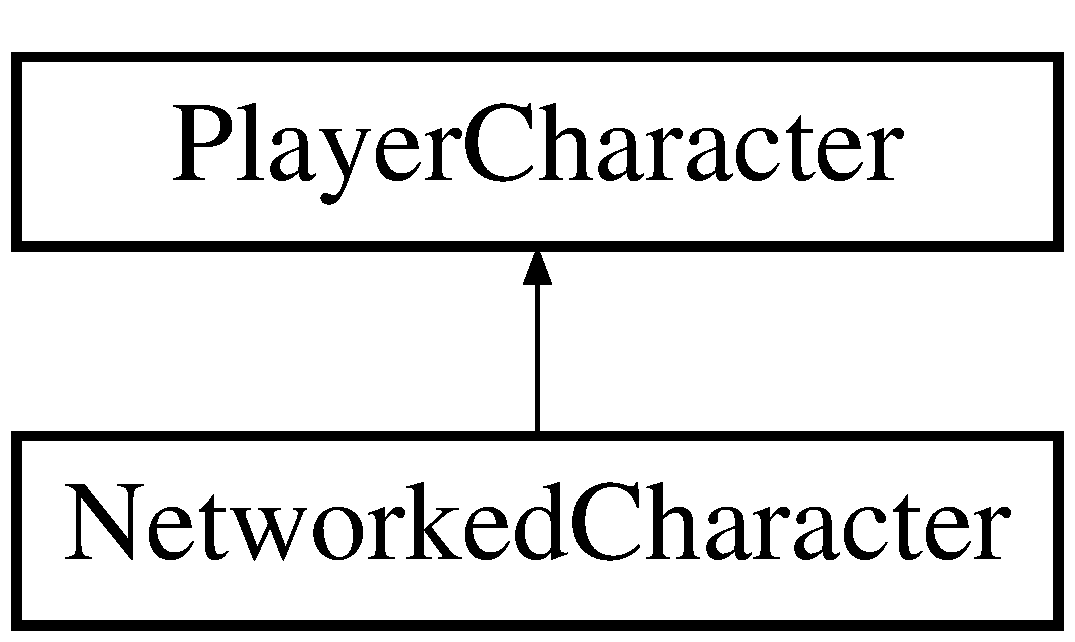
\includegraphics[height=2.000000cm]{class_networked_character}
\end{center}
\end{figure}
\subsection*{Public Member Functions}
\begin{DoxyCompactItemize}
\item 
\hyperlink{class_networked_character_ac09f304b62c04eaf431539e02b079954}{$\sim$\+Networked\+Character} ()
\item 
void \hyperlink{class_networked_character_aa445f5692ec410ff5a99ec6b6bf44e8d}{Update} (float dt, float Game\+Time)
\item 
sf\+::\+Ip\+Address \hyperlink{class_networked_character_a9b423c8353b00079e1c954704779ab31}{Get\+IP} ()
\item 
void \hyperlink{class_networked_character_a14c6d02226b324fa689dd758da7dcb34}{Set\+IP} (sf\+::\+Ip\+Address IP)
\item 
unsigned short \hyperlink{class_networked_character_af53749e10edfbbdb5ccbccd238d27091}{Get\+The\+Port} ()
\item 
void \hyperlink{class_networked_character_a306f2c2261fcdadbf53c7fadf3e85bdb}{Set\+The\+Port} (unsigned short Port)
\item 
void \hyperlink{class_networked_character_a41e76bfe05d14ebc9237031d149d6d0c}{Set\+Dir} (\hyperlink{_player_character_8h_af5420be377752b383864a169dfd7ba10}{Player\+Direction} Dir)
\item 
void \hyperlink{class_networked_character_a86f4c6a48fa251382bfd3d19872d4eb5}{Set\+Server\+Latency} (float Server\+Lat)
\item 
float \hyperlink{class_networked_character_a7692307cee60a4dec44a2a70f4b9f2c7}{Get\+Server\+Latency} ()
\item 
void \hyperlink{class_networked_character_a05c2f04191c8adc6dc733858403a39dd}{Add\+To\+Prediction\+List} (float x, float y, float Time\+Stamp, sf\+::\+Clock $\ast$Clock, float CurrentX, float CurrentY)
\end{DoxyCompactItemize}
\subsection*{Additional Inherited Members}


\subsection{Detailed Description}
The Networked Character

The Net\+Worked Character will represent other players on the network playing the game For each client (Host included) the P\+L\+A\+Y\+ER chacter will represent the locally controlled character The clients own player character will control movements and updates that are then sent to the host The host will transmite all player changes to the clients When this packet is recieved it will update the N\+E\+T\+W\+O\+RK characters on the clients

Essentially the Network Characters on clients will only Render other players and predict movement The Host will use these characters to control the game (whether a player is hit etc) And transmit this info to the clients 

\subsection{Constructor \& Destructor Documentation}
\hypertarget{class_networked_character_ac09f304b62c04eaf431539e02b079954}{}\label{class_networked_character_ac09f304b62c04eaf431539e02b079954} 
\index{Networked\+Character@{Networked\+Character}!````~Networked\+Character@{$\sim$\+Networked\+Character}}
\index{````~Networked\+Character@{$\sim$\+Networked\+Character}!Networked\+Character@{Networked\+Character}}
\subsubsection{\texorpdfstring{$\sim$\+Networked\+Character()}{~NetworkedCharacter()}}
{\footnotesize\ttfamily Networked\+Character\+::$\sim$\+Networked\+Character (\begin{DoxyParamCaption}{ }\end{DoxyParamCaption})}



\subsection{Member Function Documentation}
\hypertarget{class_networked_character_a05c2f04191c8adc6dc733858403a39dd}{}\label{class_networked_character_a05c2f04191c8adc6dc733858403a39dd} 
\index{Networked\+Character@{Networked\+Character}!Add\+To\+Prediction\+List@{Add\+To\+Prediction\+List}}
\index{Add\+To\+Prediction\+List@{Add\+To\+Prediction\+List}!Networked\+Character@{Networked\+Character}}
\subsubsection{\texorpdfstring{Add\+To\+Prediction\+List()}{AddToPredictionList()}}
{\footnotesize\ttfamily void Networked\+Character\+::\+Add\+To\+Prediction\+List (\begin{DoxyParamCaption}\item[{float}]{x,  }\item[{float}]{y,  }\item[{float}]{Time\+Stamp,  }\item[{sf\+::\+Clock $\ast$}]{Clock,  }\item[{float}]{CurrentX,  }\item[{float}]{CurrentY }\end{DoxyParamCaption})}

When an update is recieved it is added to the list of positons -\/ keeping track of the latest 3


\begin{DoxyParams}{Parameters}
{\em the} & x positon of the character \\
\hline
{\em the} & y positon of the character \\
\hline
{\em the} & time the message was recieved \\
\hline
{\em the} & Clock -\/ depreciated -\/ really should update this instead of writing this comment \\
\hline
{\em Current} & X and Current Y -\/ current positon of the character \\
\hline
\end{DoxyParams}
\hypertarget{class_networked_character_a9b423c8353b00079e1c954704779ab31}{}\label{class_networked_character_a9b423c8353b00079e1c954704779ab31} 
\index{Networked\+Character@{Networked\+Character}!Get\+IP@{Get\+IP}}
\index{Get\+IP@{Get\+IP}!Networked\+Character@{Networked\+Character}}
\subsubsection{\texorpdfstring{Get\+I\+P()}{GetIP()}}
{\footnotesize\ttfamily sf\+::\+Ip\+Address Networked\+Character\+::\+Get\+IP (\begin{DoxyParamCaption}{ }\end{DoxyParamCaption})\hspace{0.3cm}{\ttfamily [inline]}}

Getter and Setters for the IP of the networked Character \hypertarget{class_networked_character_a7692307cee60a4dec44a2a70f4b9f2c7}{}\label{class_networked_character_a7692307cee60a4dec44a2a70f4b9f2c7} 
\index{Networked\+Character@{Networked\+Character}!Get\+Server\+Latency@{Get\+Server\+Latency}}
\index{Get\+Server\+Latency@{Get\+Server\+Latency}!Networked\+Character@{Networked\+Character}}
\subsubsection{\texorpdfstring{Get\+Server\+Latency()}{GetServerLatency()}}
{\footnotesize\ttfamily float Networked\+Character\+::\+Get\+Server\+Latency (\begin{DoxyParamCaption}{ }\end{DoxyParamCaption})\hspace{0.3cm}{\ttfamily [inline]}}

\hypertarget{class_networked_character_af53749e10edfbbdb5ccbccd238d27091}{}\label{class_networked_character_af53749e10edfbbdb5ccbccd238d27091} 
\index{Networked\+Character@{Networked\+Character}!Get\+The\+Port@{Get\+The\+Port}}
\index{Get\+The\+Port@{Get\+The\+Port}!Networked\+Character@{Networked\+Character}}
\subsubsection{\texorpdfstring{Get\+The\+Port()}{GetThePort()}}
{\footnotesize\ttfamily unsigned short Networked\+Character\+::\+Get\+The\+Port (\begin{DoxyParamCaption}{ }\end{DoxyParamCaption})\hspace{0.3cm}{\ttfamily [inline]}}

Getters and Setters for the Port of the networked Character \hypertarget{class_networked_character_a41e76bfe05d14ebc9237031d149d6d0c}{}\label{class_networked_character_a41e76bfe05d14ebc9237031d149d6d0c} 
\index{Networked\+Character@{Networked\+Character}!Set\+Dir@{Set\+Dir}}
\index{Set\+Dir@{Set\+Dir}!Networked\+Character@{Networked\+Character}}
\subsubsection{\texorpdfstring{Set\+Dir()}{SetDir()}}
{\footnotesize\ttfamily void Networked\+Character\+::\+Set\+Dir (\begin{DoxyParamCaption}\item[{\hyperlink{_player_character_8h_af5420be377752b383864a169dfd7ba10}{Player\+Direction}}]{Dir }\end{DoxyParamCaption})\hspace{0.3cm}{\ttfamily [inline]}}

Directional Setter \hypertarget{class_networked_character_a14c6d02226b324fa689dd758da7dcb34}{}\label{class_networked_character_a14c6d02226b324fa689dd758da7dcb34} 
\index{Networked\+Character@{Networked\+Character}!Set\+IP@{Set\+IP}}
\index{Set\+IP@{Set\+IP}!Networked\+Character@{Networked\+Character}}
\subsubsection{\texorpdfstring{Set\+I\+P()}{SetIP()}}
{\footnotesize\ttfamily void Networked\+Character\+::\+Set\+IP (\begin{DoxyParamCaption}\item[{sf\+::\+Ip\+Address}]{IP }\end{DoxyParamCaption})\hspace{0.3cm}{\ttfamily [inline]}}

\hypertarget{class_networked_character_a86f4c6a48fa251382bfd3d19872d4eb5}{}\label{class_networked_character_a86f4c6a48fa251382bfd3d19872d4eb5} 
\index{Networked\+Character@{Networked\+Character}!Set\+Server\+Latency@{Set\+Server\+Latency}}
\index{Set\+Server\+Latency@{Set\+Server\+Latency}!Networked\+Character@{Networked\+Character}}
\subsubsection{\texorpdfstring{Set\+Server\+Latency()}{SetServerLatency()}}
{\footnotesize\ttfamily void Networked\+Character\+::\+Set\+Server\+Latency (\begin{DoxyParamCaption}\item[{float}]{Server\+Lat }\end{DoxyParamCaption})\hspace{0.3cm}{\ttfamily [inline]}}

I dont use these functions.... \hypertarget{class_networked_character_a306f2c2261fcdadbf53c7fadf3e85bdb}{}\label{class_networked_character_a306f2c2261fcdadbf53c7fadf3e85bdb} 
\index{Networked\+Character@{Networked\+Character}!Set\+The\+Port@{Set\+The\+Port}}
\index{Set\+The\+Port@{Set\+The\+Port}!Networked\+Character@{Networked\+Character}}
\subsubsection{\texorpdfstring{Set\+The\+Port()}{SetThePort()}}
{\footnotesize\ttfamily void Networked\+Character\+::\+Set\+The\+Port (\begin{DoxyParamCaption}\item[{unsigned short}]{Port }\end{DoxyParamCaption})\hspace{0.3cm}{\ttfamily [inline]}}

\hypertarget{class_networked_character_aa445f5692ec410ff5a99ec6b6bf44e8d}{}\label{class_networked_character_aa445f5692ec410ff5a99ec6b6bf44e8d} 
\index{Networked\+Character@{Networked\+Character}!Update@{Update}}
\index{Update@{Update}!Networked\+Character@{Networked\+Character}}
\subsubsection{\texorpdfstring{Update()}{Update()}}
{\footnotesize\ttfamily void Networked\+Character\+::\+Update (\begin{DoxyParamCaption}\item[{float}]{dt,  }\item[{float}]{Game\+Time }\end{DoxyParamCaption})}

Updates the Networked Character Prediciton happens here


\begin{DoxyParams}{Parameters}
{\em Delta} & Time \\
\hline
{\em the} & current game time \\
\hline
\end{DoxyParams}


The documentation for this class was generated from the following files\+:\begin{DoxyCompactItemize}
\item 
E\+:/\+Coding/\+S\+F\+M\+L\+\_\+\+Networked\+Game/\+Networking\+Coursework/\hyperlink{_networked_character_8h}{Networked\+Character.\+h}\item 
E\+:/\+Coding/\+S\+F\+M\+L\+\_\+\+Networked\+Game/\+Networking\+Coursework/\hyperlink{_networked_character_8cpp}{Networked\+Character.\+cpp}\end{DoxyCompactItemize}

\hypertarget{class_player_character}{}\section{Player\+Character Class Reference}
\label{class_player_character}\index{Player\+Character@{Player\+Character}}


{\ttfamily \#include $<$Player\+Character.\+h$>$}

Inheritance diagram for Player\+Character\+:\begin{figure}[H]
\begin{center}
\leavevmode
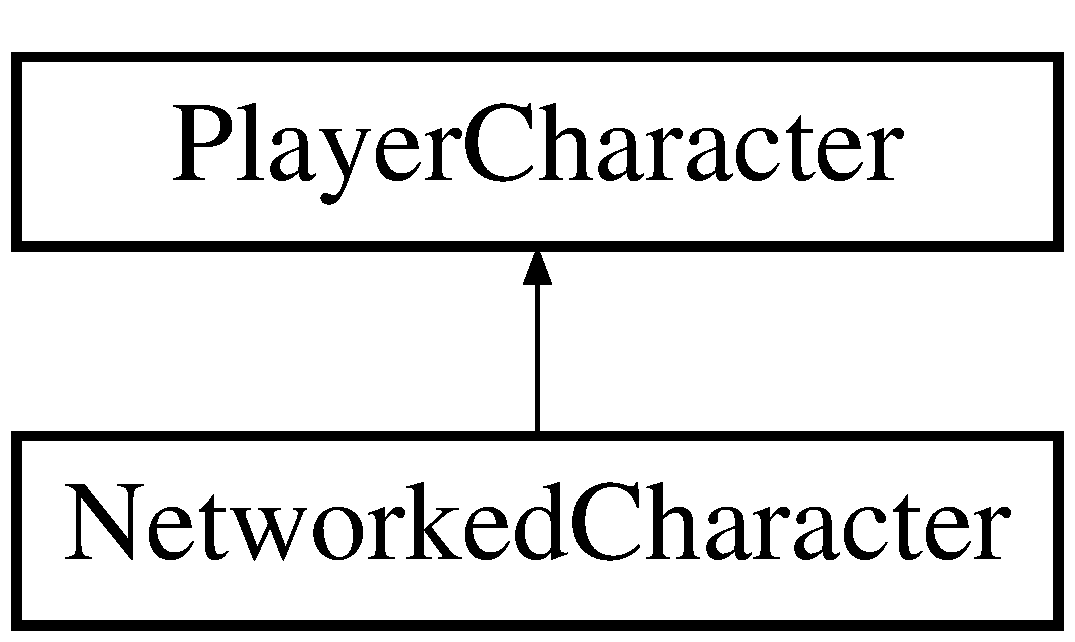
\includegraphics[height=2.000000cm]{class_player_character}
\end{center}
\end{figure}
\subsection*{Public Member Functions}
\begin{DoxyCompactItemize}
\item 
\hyperlink{class_player_character_af3ac12a41f58d860fb716138578bd95f}{Player\+Character} ()
\item 
\hyperlink{class_player_character_a4915330a9f743156b6860a97e6d68e28}{$\sim$\+Player\+Character} ()
\item 
void \hyperlink{class_player_character_a780111b98376a28607aa21207b4cf91a}{Init} (int Player\+ID, \hyperlink{_player_character_8h_a3fe9312ea357fba2db18ae32ffe5bca1}{Player\+Colour} Colour, sf\+::\+Vector2f Starting\+Pos, std\+::string Filename, \hyperlink{class_debug_u_i}{Debug\+UI} \&Debug\+Screen)
\item 
virtual void \hyperlink{class_player_character_a94bbe2b48d72236a6de6cb88f492da76}{Update} (float dt)
\item 
bool \hyperlink{class_player_character_a19081e3c59bc962efb9c5e2c7887c267}{Bomb\+Requests} (float dt, float Game\+Time)
\item 
void \hyperlink{class_player_character_af46ba459570710dcca3bfd6edb0cb7f8}{Render} (sf\+::\+Render\+Window $\ast$Window)
\item 
sf\+::\+Uint32 \hyperlink{class_player_character_a0c4259c1a2eec6c1669bf9ce9ff4a646}{Get\+Colour} ()
\item 
float \hyperlink{class_player_character_aaa03186b913d3ff5673dcde280284bf5}{Get\+X\+Pos} ()
\item 
float \hyperlink{class_player_character_a666a4e7b2a642704d7435beaccb89e6a}{Get\+Y\+Pos} ()
\item 
sf\+::\+Uint8 \hyperlink{class_player_character_aa7be8bfe26290d285725f0035de6e31c}{Get\+ID} ()
\item 
sf\+::\+Uint8 \hyperlink{class_player_character_af6704dd235bd347fb3f2c59a56015b51}{Get\+Dir} ()
\item 
float \hyperlink{class_player_character_a116a731d0dd7788b0e8b8100cd97928a}{Get\+Bomb\+Explosion\+Delay} ()
\end{DoxyCompactItemize}
\subsection*{Protected Member Functions}
\begin{DoxyCompactItemize}
\item 
virtual void \hyperlink{class_player_character_a46f4559ce3efcab6bdd807ea2446fdfa}{Movement} (float dt)
\item 
void \hyperlink{class_player_character_ac465108f9f9337aba263be0676bed00b}{Update\+Sprite} (int Sprite\+Pos, float dt)
\item 
void \hyperlink{class_player_character_a9891ba485885beb2516f632a0a252e19}{Update\+Sprite\+State} (float dt)
\end{DoxyCompactItemize}
\subsection*{Protected Attributes}
\begin{DoxyCompactItemize}
\item 
sf\+::\+Clock \hyperlink{class_player_character_a8fa9ea765016a1b910ab7007f2071edb}{m\+\_\+\+Bomb\+Clock}
\item 
float \hyperlink{class_player_character_ad8ccf5c2e03d93085bacaf60f2801fb7}{m\+\_\+\+Bomb\+Fire\+Rate}
\item 
float \hyperlink{class_player_character_a1f8732b219730a15a1666ec77e690a71}{m\+\_\+\+Bomb\+Explosion\+Delay}
\item 
sf\+::\+Texture \hyperlink{class_player_character_a0536f6e9f31ba651a9e207d88227f7b9}{m\+\_\+\+Texture}
\item 
sf\+::\+Sprite \hyperlink{class_player_character_a65d271da64e077967d283b37396d1549}{m\+\_\+\+Sprite}
\item 
int \hyperlink{class_player_character_aa71fe75fed5e2e7da416b8073f9b37da}{m\+\_\+\+Texture\+\_\+\+Width}
\item 
int \hyperlink{class_player_character_a544274318c87093392e763ecaee909d6}{m\+\_\+\+Texture\+\_\+\+Height}
\item 
int \hyperlink{class_player_character_a8bf6864a7377ccafda31172a6e5b009d}{m\+\_\+\+Sprite\+\_\+\+X\+\_\+\+Pos}
\item 
int \hyperlink{class_player_character_aea5fde273dee8afe18af848cc7865b50}{m\+\_\+\+Sprite\+\_\+\+Y\+\_\+\+Pos}
\item 
sf\+::\+Uint8 \hyperlink{class_player_character_ab3ae00b8837356dd6bdb86d90a941cad}{m\+\_\+\+ID}
\item 
\hyperlink{_player_character_8h_a3fe9312ea357fba2db18ae32ffe5bca1}{Player\+Colour} \hyperlink{class_player_character_ab1d44ae0ba6b9067f771fb9bc15a5a3b}{m\+\_\+\+Colour}
\item 
float \hyperlink{class_player_character_af4dcd4c48904565edaad6274897991a8}{m\+\_\+\+Speed}
\item 
\hyperlink{class_debug_u_i}{Debug\+UI} $\ast$ \hyperlink{class_player_character_ad4c2a95040c945081107dd20d2634137}{m\+\_\+\+Debug}
\item 
sf\+::\+Text $\ast$ \hyperlink{class_player_character_afd9f0e8831f894c5e621543ed3ff3d9c}{Player\+Position\+Text}
\item 
sf\+::\+Vector2f \hyperlink{class_player_character_a551aaac5dacaebbde21c5b6d46f5ec7d}{m\+\_\+\+Position}
\item 
float \hyperlink{class_player_character_a45f3c61083c1db2753500d8e217ca463}{m\+\_\+\+Frames\+Per\+Second}
\item 
float \hyperlink{class_player_character_accc3a138e2f16b4fd7e07637fa00ef78}{m\+\_\+\+Anim\+Counter}
\item 
int \hyperlink{class_player_character_aef80914837c7107dd3e9b8315c913160}{m\+\_\+\+Current\+Sprite\+Pos}
\item 
\hyperlink{_player_character_8h_af5420be377752b383864a169dfd7ba10}{Player\+Direction} \hyperlink{class_player_character_ac2d756b41be615f4fa31cbb99d405109}{m\+\_\+\+Dir}
\item 
bool \hyperlink{class_player_character_a2c8e033c4db7139172041a4476ef1534}{m\+\_\+\+Do\+Once}
\end{DoxyCompactItemize}


\subsection{Detailed Description}
The Player Character

The Player Character is a player game object that can be controlled by the local user The Directional Pad controls movement and changes the player state. Also controls if the player can place bombs and interaction in the game This object will be accessed to get positon for sending to other clients 

\subsection{Constructor \& Destructor Documentation}
\hypertarget{class_player_character_af3ac12a41f58d860fb716138578bd95f}{}\label{class_player_character_af3ac12a41f58d860fb716138578bd95f} 
\index{Player\+Character@{Player\+Character}!Player\+Character@{Player\+Character}}
\index{Player\+Character@{Player\+Character}!Player\+Character@{Player\+Character}}
\subsubsection{\texorpdfstring{Player\+Character()}{PlayerCharacter()}}
{\footnotesize\ttfamily Player\+Character\+::\+Player\+Character (\begin{DoxyParamCaption}{ }\end{DoxyParamCaption})}

\hypertarget{class_player_character_a4915330a9f743156b6860a97e6d68e28}{}\label{class_player_character_a4915330a9f743156b6860a97e6d68e28} 
\index{Player\+Character@{Player\+Character}!````~Player\+Character@{$\sim$\+Player\+Character}}
\index{````~Player\+Character@{$\sim$\+Player\+Character}!Player\+Character@{Player\+Character}}
\subsubsection{\texorpdfstring{$\sim$\+Player\+Character()}{~PlayerCharacter()}}
{\footnotesize\ttfamily Player\+Character\+::$\sim$\+Player\+Character (\begin{DoxyParamCaption}{ }\end{DoxyParamCaption})}



\subsection{Member Function Documentation}
\hypertarget{class_player_character_a19081e3c59bc962efb9c5e2c7887c267}{}\label{class_player_character_a19081e3c59bc962efb9c5e2c7887c267} 
\index{Player\+Character@{Player\+Character}!Bomb\+Requests@{Bomb\+Requests}}
\index{Bomb\+Requests@{Bomb\+Requests}!Player\+Character@{Player\+Character}}
\subsubsection{\texorpdfstring{Bomb\+Requests()}{BombRequests()}}
{\footnotesize\ttfamily bool Player\+Character\+::\+Bomb\+Requests (\begin{DoxyParamCaption}\item[{float}]{dt,  }\item[{float}]{Game\+Time }\end{DoxyParamCaption})}

\hyperlink{class_bomb}{Bomb} Requests

Controlls whether tha player can set bombs


\begin{DoxyParams}{Parameters}
{\em delta} & time \\
\hline
{\em the} & current game time \\
\hline
\end{DoxyParams}
\begin{DoxyReturn}{Returns}
returns true if the player plants a bomb 
\end{DoxyReturn}
\hypertarget{class_player_character_a116a731d0dd7788b0e8b8100cd97928a}{}\label{class_player_character_a116a731d0dd7788b0e8b8100cd97928a} 
\index{Player\+Character@{Player\+Character}!Get\+Bomb\+Explosion\+Delay@{Get\+Bomb\+Explosion\+Delay}}
\index{Get\+Bomb\+Explosion\+Delay@{Get\+Bomb\+Explosion\+Delay}!Player\+Character@{Player\+Character}}
\subsubsection{\texorpdfstring{Get\+Bomb\+Explosion\+Delay()}{GetBombExplosionDelay()}}
{\footnotesize\ttfamily float Player\+Character\+::\+Get\+Bomb\+Explosion\+Delay (\begin{DoxyParamCaption}{ }\end{DoxyParamCaption})\hspace{0.3cm}{\ttfamily [inline]}}

Gets the delay set for each bomb Plan would be that different power ups could increase/decrease bombs \hypertarget{class_player_character_a0c4259c1a2eec6c1669bf9ce9ff4a646}{}\label{class_player_character_a0c4259c1a2eec6c1669bf9ce9ff4a646} 
\index{Player\+Character@{Player\+Character}!Get\+Colour@{Get\+Colour}}
\index{Get\+Colour@{Get\+Colour}!Player\+Character@{Player\+Character}}
\subsubsection{\texorpdfstring{Get\+Colour()}{GetColour()}}
{\footnotesize\ttfamily sf\+::\+Uint32 Player\+Character\+::\+Get\+Colour (\begin{DoxyParamCaption}{ }\end{DoxyParamCaption})\hspace{0.3cm}{\ttfamily [inline]}}

Getter for the player colour \hypertarget{class_player_character_af6704dd235bd347fb3f2c59a56015b51}{}\label{class_player_character_af6704dd235bd347fb3f2c59a56015b51} 
\index{Player\+Character@{Player\+Character}!Get\+Dir@{Get\+Dir}}
\index{Get\+Dir@{Get\+Dir}!Player\+Character@{Player\+Character}}
\subsubsection{\texorpdfstring{Get\+Dir()}{GetDir()}}
{\footnotesize\ttfamily sf\+::\+Uint8 Player\+Character\+::\+Get\+Dir (\begin{DoxyParamCaption}{ }\end{DoxyParamCaption})\hspace{0.3cm}{\ttfamily [inline]}}

Getter For the player Direction \hypertarget{class_player_character_aa7be8bfe26290d285725f0035de6e31c}{}\label{class_player_character_aa7be8bfe26290d285725f0035de6e31c} 
\index{Player\+Character@{Player\+Character}!Get\+ID@{Get\+ID}}
\index{Get\+ID@{Get\+ID}!Player\+Character@{Player\+Character}}
\subsubsection{\texorpdfstring{Get\+I\+D()}{GetID()}}
{\footnotesize\ttfamily sf\+::\+Uint8 Player\+Character\+::\+Get\+ID (\begin{DoxyParamCaption}{ }\end{DoxyParamCaption})\hspace{0.3cm}{\ttfamily [inline]}}

Getter For the player ID \hypertarget{class_player_character_aaa03186b913d3ff5673dcde280284bf5}{}\label{class_player_character_aaa03186b913d3ff5673dcde280284bf5} 
\index{Player\+Character@{Player\+Character}!Get\+X\+Pos@{Get\+X\+Pos}}
\index{Get\+X\+Pos@{Get\+X\+Pos}!Player\+Character@{Player\+Character}}
\subsubsection{\texorpdfstring{Get\+X\+Pos()}{GetXPos()}}
{\footnotesize\ttfamily float Player\+Character\+::\+Get\+X\+Pos (\begin{DoxyParamCaption}{ }\end{DoxyParamCaption})\hspace{0.3cm}{\ttfamily [inline]}}

Getters and Setters for player positions \hypertarget{class_player_character_a666a4e7b2a642704d7435beaccb89e6a}{}\label{class_player_character_a666a4e7b2a642704d7435beaccb89e6a} 
\index{Player\+Character@{Player\+Character}!Get\+Y\+Pos@{Get\+Y\+Pos}}
\index{Get\+Y\+Pos@{Get\+Y\+Pos}!Player\+Character@{Player\+Character}}
\subsubsection{\texorpdfstring{Get\+Y\+Pos()}{GetYPos()}}
{\footnotesize\ttfamily float Player\+Character\+::\+Get\+Y\+Pos (\begin{DoxyParamCaption}{ }\end{DoxyParamCaption})\hspace{0.3cm}{\ttfamily [inline]}}

\hypertarget{class_player_character_a780111b98376a28607aa21207b4cf91a}{}\label{class_player_character_a780111b98376a28607aa21207b4cf91a} 
\index{Player\+Character@{Player\+Character}!Init@{Init}}
\index{Init@{Init}!Player\+Character@{Player\+Character}}
\subsubsection{\texorpdfstring{Init()}{Init()}}
{\footnotesize\ttfamily void Player\+Character\+::\+Init (\begin{DoxyParamCaption}\item[{int}]{Player\+ID,  }\item[{\hyperlink{_player_character_8h_a3fe9312ea357fba2db18ae32ffe5bca1}{Player\+Colour}}]{Colour,  }\item[{sf\+::\+Vector2f}]{Starting\+Pos,  }\item[{std\+::string}]{Filename,  }\item[{\hyperlink{class_debug_u_i}{Debug\+UI} \&}]{Debug\+Screen }\end{DoxyParamCaption})}

The Initialiser for the player character


\begin{DoxyParams}{Parameters}
{\em Player} & Id that was given by the host \\
\hline
{\em The} & selected player colour \\
\hline
{\em The} & starting position \\
\hline
{\em the} & Filename location the textures for the player  to the debug screen for adding messages \\
\hline
\end{DoxyParams}
\hypertarget{class_player_character_a46f4559ce3efcab6bdd807ea2446fdfa}{}\label{class_player_character_a46f4559ce3efcab6bdd807ea2446fdfa} 
\index{Player\+Character@{Player\+Character}!Movement@{Movement}}
\index{Movement@{Movement}!Player\+Character@{Player\+Character}}
\subsubsection{\texorpdfstring{Movement()}{Movement()}}
{\footnotesize\ttfamily void Player\+Character\+::\+Movement (\begin{DoxyParamCaption}\item[{float}]{dt }\end{DoxyParamCaption})\hspace{0.3cm}{\ttfamily [protected]}, {\ttfamily [virtual]}}

Updates the movement of the player character


\begin{DoxyParams}{Parameters}
{\em Delta} & time \\
\hline
\end{DoxyParams}
\hypertarget{class_player_character_af46ba459570710dcca3bfd6edb0cb7f8}{}\label{class_player_character_af46ba459570710dcca3bfd6edb0cb7f8} 
\index{Player\+Character@{Player\+Character}!Render@{Render}}
\index{Render@{Render}!Player\+Character@{Player\+Character}}
\subsubsection{\texorpdfstring{Render()}{Render()}}
{\footnotesize\ttfamily void Player\+Character\+::\+Render (\begin{DoxyParamCaption}\item[{sf\+::\+Render\+Window $\ast$}]{Window }\end{DoxyParamCaption})}

The Render Function


\begin{DoxyParams}{Parameters}
{\em Pointer} & to the S\+F\+ML window \\
\hline
\end{DoxyParams}
\hypertarget{class_player_character_a94bbe2b48d72236a6de6cb88f492da76}{}\label{class_player_character_a94bbe2b48d72236a6de6cb88f492da76} 
\index{Player\+Character@{Player\+Character}!Update@{Update}}
\index{Update@{Update}!Player\+Character@{Player\+Character}}
\subsubsection{\texorpdfstring{Update()}{Update()}}
{\footnotesize\ttfamily void Player\+Character\+::\+Update (\begin{DoxyParamCaption}\item[{float}]{dt }\end{DoxyParamCaption})\hspace{0.3cm}{\ttfamily [virtual]}}

Update Function


\begin{DoxyParams}{Parameters}
{\em Delta} & Time \\
\hline
\end{DoxyParams}
\hypertarget{class_player_character_ac465108f9f9337aba263be0676bed00b}{}\label{class_player_character_ac465108f9f9337aba263be0676bed00b} 
\index{Player\+Character@{Player\+Character}!Update\+Sprite@{Update\+Sprite}}
\index{Update\+Sprite@{Update\+Sprite}!Player\+Character@{Player\+Character}}
\subsubsection{\texorpdfstring{Update\+Sprite()}{UpdateSprite()}}
{\footnotesize\ttfamily void Player\+Character\+::\+Update\+Sprite (\begin{DoxyParamCaption}\item[{int}]{Sprite\+Pos,  }\item[{float}]{dt }\end{DoxyParamCaption})\hspace{0.3cm}{\ttfamily [protected]}}

Animates the sprirte


\begin{DoxyParams}{Parameters}
{\em the} & position of the sprite to be at on the texture (Starting animation point) \\
\hline
{\em delta} & time \\
\hline
\end{DoxyParams}
\hypertarget{class_player_character_a9891ba485885beb2516f632a0a252e19}{}\label{class_player_character_a9891ba485885beb2516f632a0a252e19} 
\index{Player\+Character@{Player\+Character}!Update\+Sprite\+State@{Update\+Sprite\+State}}
\index{Update\+Sprite\+State@{Update\+Sprite\+State}!Player\+Character@{Player\+Character}}
\subsubsection{\texorpdfstring{Update\+Sprite\+State()}{UpdateSpriteState()}}
{\footnotesize\ttfamily void Player\+Character\+::\+Update\+Sprite\+State (\begin{DoxyParamCaption}\item[{float}]{dt }\end{DoxyParamCaption})\hspace{0.3cm}{\ttfamily [protected]}}

Updates the current state of the sprite (Controlled by the direction the player is moving)


\begin{DoxyParams}{Parameters}
{\em delta} & time \\
\hline
\end{DoxyParams}


\subsection{Member Data Documentation}
\hypertarget{class_player_character_accc3a138e2f16b4fd7e07637fa00ef78}{}\label{class_player_character_accc3a138e2f16b4fd7e07637fa00ef78} 
\index{Player\+Character@{Player\+Character}!m\+\_\+\+Anim\+Counter@{m\+\_\+\+Anim\+Counter}}
\index{m\+\_\+\+Anim\+Counter@{m\+\_\+\+Anim\+Counter}!Player\+Character@{Player\+Character}}
\subsubsection{\texorpdfstring{m\+\_\+\+Anim\+Counter}{m\_AnimCounter}}
{\footnotesize\ttfamily float Player\+Character\+::m\+\_\+\+Anim\+Counter\hspace{0.3cm}{\ttfamily [protected]}}

\hypertarget{class_player_character_a8fa9ea765016a1b910ab7007f2071edb}{}\label{class_player_character_a8fa9ea765016a1b910ab7007f2071edb} 
\index{Player\+Character@{Player\+Character}!m\+\_\+\+Bomb\+Clock@{m\+\_\+\+Bomb\+Clock}}
\index{m\+\_\+\+Bomb\+Clock@{m\+\_\+\+Bomb\+Clock}!Player\+Character@{Player\+Character}}
\subsubsection{\texorpdfstring{m\+\_\+\+Bomb\+Clock}{m\_BombClock}}
{\footnotesize\ttfamily sf\+::\+Clock Player\+Character\+::m\+\_\+\+Bomb\+Clock\hspace{0.3cm}{\ttfamily [protected]}}

Members controlling the bomb timer/times \hypertarget{class_player_character_a1f8732b219730a15a1666ec77e690a71}{}\label{class_player_character_a1f8732b219730a15a1666ec77e690a71} 
\index{Player\+Character@{Player\+Character}!m\+\_\+\+Bomb\+Explosion\+Delay@{m\+\_\+\+Bomb\+Explosion\+Delay}}
\index{m\+\_\+\+Bomb\+Explosion\+Delay@{m\+\_\+\+Bomb\+Explosion\+Delay}!Player\+Character@{Player\+Character}}
\subsubsection{\texorpdfstring{m\+\_\+\+Bomb\+Explosion\+Delay}{m\_BombExplosionDelay}}
{\footnotesize\ttfamily float Player\+Character\+::m\+\_\+\+Bomb\+Explosion\+Delay\hspace{0.3cm}{\ttfamily [protected]}}

\hypertarget{class_player_character_ad8ccf5c2e03d93085bacaf60f2801fb7}{}\label{class_player_character_ad8ccf5c2e03d93085bacaf60f2801fb7} 
\index{Player\+Character@{Player\+Character}!m\+\_\+\+Bomb\+Fire\+Rate@{m\+\_\+\+Bomb\+Fire\+Rate}}
\index{m\+\_\+\+Bomb\+Fire\+Rate@{m\+\_\+\+Bomb\+Fire\+Rate}!Player\+Character@{Player\+Character}}
\subsubsection{\texorpdfstring{m\+\_\+\+Bomb\+Fire\+Rate}{m\_BombFireRate}}
{\footnotesize\ttfamily float Player\+Character\+::m\+\_\+\+Bomb\+Fire\+Rate\hspace{0.3cm}{\ttfamily [protected]}}

\hypertarget{class_player_character_ab1d44ae0ba6b9067f771fb9bc15a5a3b}{}\label{class_player_character_ab1d44ae0ba6b9067f771fb9bc15a5a3b} 
\index{Player\+Character@{Player\+Character}!m\+\_\+\+Colour@{m\+\_\+\+Colour}}
\index{m\+\_\+\+Colour@{m\+\_\+\+Colour}!Player\+Character@{Player\+Character}}
\subsubsection{\texorpdfstring{m\+\_\+\+Colour}{m\_Colour}}
{\footnotesize\ttfamily \hyperlink{_player_character_8h_a3fe9312ea357fba2db18ae32ffe5bca1}{Player\+Colour} Player\+Character\+::m\+\_\+\+Colour\hspace{0.3cm}{\ttfamily [protected]}}

\hypertarget{class_player_character_aef80914837c7107dd3e9b8315c913160}{}\label{class_player_character_aef80914837c7107dd3e9b8315c913160} 
\index{Player\+Character@{Player\+Character}!m\+\_\+\+Current\+Sprite\+Pos@{m\+\_\+\+Current\+Sprite\+Pos}}
\index{m\+\_\+\+Current\+Sprite\+Pos@{m\+\_\+\+Current\+Sprite\+Pos}!Player\+Character@{Player\+Character}}
\subsubsection{\texorpdfstring{m\+\_\+\+Current\+Sprite\+Pos}{m\_CurrentSpritePos}}
{\footnotesize\ttfamily int Player\+Character\+::m\+\_\+\+Current\+Sprite\+Pos\hspace{0.3cm}{\ttfamily [protected]}}

\hypertarget{class_player_character_ad4c2a95040c945081107dd20d2634137}{}\label{class_player_character_ad4c2a95040c945081107dd20d2634137} 
\index{Player\+Character@{Player\+Character}!m\+\_\+\+Debug@{m\+\_\+\+Debug}}
\index{m\+\_\+\+Debug@{m\+\_\+\+Debug}!Player\+Character@{Player\+Character}}
\subsubsection{\texorpdfstring{m\+\_\+\+Debug}{m\_Debug}}
{\footnotesize\ttfamily \hyperlink{class_debug_u_i}{Debug\+UI}$\ast$ Player\+Character\+::m\+\_\+\+Debug\hspace{0.3cm}{\ttfamily [protected]}}

Members controlling the debug screen/text \hypertarget{class_player_character_ac2d756b41be615f4fa31cbb99d405109}{}\label{class_player_character_ac2d756b41be615f4fa31cbb99d405109} 
\index{Player\+Character@{Player\+Character}!m\+\_\+\+Dir@{m\+\_\+\+Dir}}
\index{m\+\_\+\+Dir@{m\+\_\+\+Dir}!Player\+Character@{Player\+Character}}
\subsubsection{\texorpdfstring{m\+\_\+\+Dir}{m\_Dir}}
{\footnotesize\ttfamily \hyperlink{_player_character_8h_af5420be377752b383864a169dfd7ba10}{Player\+Direction} Player\+Character\+::m\+\_\+\+Dir\hspace{0.3cm}{\ttfamily [protected]}}

\hypertarget{class_player_character_a2c8e033c4db7139172041a4476ef1534}{}\label{class_player_character_a2c8e033c4db7139172041a4476ef1534} 
\index{Player\+Character@{Player\+Character}!m\+\_\+\+Do\+Once@{m\+\_\+\+Do\+Once}}
\index{m\+\_\+\+Do\+Once@{m\+\_\+\+Do\+Once}!Player\+Character@{Player\+Character}}
\subsubsection{\texorpdfstring{m\+\_\+\+Do\+Once}{m\_DoOnce}}
{\footnotesize\ttfamily bool Player\+Character\+::m\+\_\+\+Do\+Once\hspace{0.3cm}{\ttfamily [protected]}}

Wierd bug in S\+F\+ML that returns N\+AN when calling Get\+Sprite\+Position from the Networked Character Setting the position once from the net char seems to fix it \hypertarget{class_player_character_a45f3c61083c1db2753500d8e217ca463}{}\label{class_player_character_a45f3c61083c1db2753500d8e217ca463} 
\index{Player\+Character@{Player\+Character}!m\+\_\+\+Frames\+Per\+Second@{m\+\_\+\+Frames\+Per\+Second}}
\index{m\+\_\+\+Frames\+Per\+Second@{m\+\_\+\+Frames\+Per\+Second}!Player\+Character@{Player\+Character}}
\subsubsection{\texorpdfstring{m\+\_\+\+Frames\+Per\+Second}{m\_FramesPerSecond}}
{\footnotesize\ttfamily float Player\+Character\+::m\+\_\+\+Frames\+Per\+Second\hspace{0.3cm}{\ttfamily [protected]}}

Members controlling animation \hypertarget{class_player_character_ab3ae00b8837356dd6bdb86d90a941cad}{}\label{class_player_character_ab3ae00b8837356dd6bdb86d90a941cad} 
\index{Player\+Character@{Player\+Character}!m\+\_\+\+ID@{m\+\_\+\+ID}}
\index{m\+\_\+\+ID@{m\+\_\+\+ID}!Player\+Character@{Player\+Character}}
\subsubsection{\texorpdfstring{m\+\_\+\+ID}{m\_ID}}
{\footnotesize\ttfamily sf\+::\+Uint8 Player\+Character\+::m\+\_\+\+ID\hspace{0.3cm}{\ttfamily [protected]}}

Player Identifiers \hypertarget{class_player_character_a551aaac5dacaebbde21c5b6d46f5ec7d}{}\label{class_player_character_a551aaac5dacaebbde21c5b6d46f5ec7d} 
\index{Player\+Character@{Player\+Character}!m\+\_\+\+Position@{m\+\_\+\+Position}}
\index{m\+\_\+\+Position@{m\+\_\+\+Position}!Player\+Character@{Player\+Character}}
\subsubsection{\texorpdfstring{m\+\_\+\+Position}{m\_Position}}
{\footnotesize\ttfamily sf\+::\+Vector2f Player\+Character\+::m\+\_\+\+Position\hspace{0.3cm}{\ttfamily [protected]}}

\hypertarget{class_player_character_af4dcd4c48904565edaad6274897991a8}{}\label{class_player_character_af4dcd4c48904565edaad6274897991a8} 
\index{Player\+Character@{Player\+Character}!m\+\_\+\+Speed@{m\+\_\+\+Speed}}
\index{m\+\_\+\+Speed@{m\+\_\+\+Speed}!Player\+Character@{Player\+Character}}
\subsubsection{\texorpdfstring{m\+\_\+\+Speed}{m\_Speed}}
{\footnotesize\ttfamily float Player\+Character\+::m\+\_\+\+Speed\hspace{0.3cm}{\ttfamily [protected]}}

Speed in which player can move \hypertarget{class_player_character_a65d271da64e077967d283b37396d1549}{}\label{class_player_character_a65d271da64e077967d283b37396d1549} 
\index{Player\+Character@{Player\+Character}!m\+\_\+\+Sprite@{m\+\_\+\+Sprite}}
\index{m\+\_\+\+Sprite@{m\+\_\+\+Sprite}!Player\+Character@{Player\+Character}}
\subsubsection{\texorpdfstring{m\+\_\+\+Sprite}{m\_Sprite}}
{\footnotesize\ttfamily sf\+::\+Sprite Player\+Character\+::m\+\_\+\+Sprite\hspace{0.3cm}{\ttfamily [protected]}}

\hypertarget{class_player_character_a8bf6864a7377ccafda31172a6e5b009d}{}\label{class_player_character_a8bf6864a7377ccafda31172a6e5b009d} 
\index{Player\+Character@{Player\+Character}!m\+\_\+\+Sprite\+\_\+\+X\+\_\+\+Pos@{m\+\_\+\+Sprite\+\_\+\+X\+\_\+\+Pos}}
\index{m\+\_\+\+Sprite\+\_\+\+X\+\_\+\+Pos@{m\+\_\+\+Sprite\+\_\+\+X\+\_\+\+Pos}!Player\+Character@{Player\+Character}}
\subsubsection{\texorpdfstring{m\+\_\+\+Sprite\+\_\+\+X\+\_\+\+Pos}{m\_Sprite\_X\_Pos}}
{\footnotesize\ttfamily int Player\+Character\+::m\+\_\+\+Sprite\+\_\+\+X\+\_\+\+Pos\hspace{0.3cm}{\ttfamily [protected]}}

\hypertarget{class_player_character_aea5fde273dee8afe18af848cc7865b50}{}\label{class_player_character_aea5fde273dee8afe18af848cc7865b50} 
\index{Player\+Character@{Player\+Character}!m\+\_\+\+Sprite\+\_\+\+Y\+\_\+\+Pos@{m\+\_\+\+Sprite\+\_\+\+Y\+\_\+\+Pos}}
\index{m\+\_\+\+Sprite\+\_\+\+Y\+\_\+\+Pos@{m\+\_\+\+Sprite\+\_\+\+Y\+\_\+\+Pos}!Player\+Character@{Player\+Character}}
\subsubsection{\texorpdfstring{m\+\_\+\+Sprite\+\_\+\+Y\+\_\+\+Pos}{m\_Sprite\_Y\_Pos}}
{\footnotesize\ttfamily int Player\+Character\+::m\+\_\+\+Sprite\+\_\+\+Y\+\_\+\+Pos\hspace{0.3cm}{\ttfamily [protected]}}

\hypertarget{class_player_character_a0536f6e9f31ba651a9e207d88227f7b9}{}\label{class_player_character_a0536f6e9f31ba651a9e207d88227f7b9} 
\index{Player\+Character@{Player\+Character}!m\+\_\+\+Texture@{m\+\_\+\+Texture}}
\index{m\+\_\+\+Texture@{m\+\_\+\+Texture}!Player\+Character@{Player\+Character}}
\subsubsection{\texorpdfstring{m\+\_\+\+Texture}{m\_Texture}}
{\footnotesize\ttfamily sf\+::\+Texture Player\+Character\+::m\+\_\+\+Texture\hspace{0.3cm}{\ttfamily [protected]}}

Members controlling sprite and animation \hypertarget{class_player_character_a544274318c87093392e763ecaee909d6}{}\label{class_player_character_a544274318c87093392e763ecaee909d6} 
\index{Player\+Character@{Player\+Character}!m\+\_\+\+Texture\+\_\+\+Height@{m\+\_\+\+Texture\+\_\+\+Height}}
\index{m\+\_\+\+Texture\+\_\+\+Height@{m\+\_\+\+Texture\+\_\+\+Height}!Player\+Character@{Player\+Character}}
\subsubsection{\texorpdfstring{m\+\_\+\+Texture\+\_\+\+Height}{m\_Texture\_Height}}
{\footnotesize\ttfamily int Player\+Character\+::m\+\_\+\+Texture\+\_\+\+Height\hspace{0.3cm}{\ttfamily [protected]}}

\hypertarget{class_player_character_aa71fe75fed5e2e7da416b8073f9b37da}{}\label{class_player_character_aa71fe75fed5e2e7da416b8073f9b37da} 
\index{Player\+Character@{Player\+Character}!m\+\_\+\+Texture\+\_\+\+Width@{m\+\_\+\+Texture\+\_\+\+Width}}
\index{m\+\_\+\+Texture\+\_\+\+Width@{m\+\_\+\+Texture\+\_\+\+Width}!Player\+Character@{Player\+Character}}
\subsubsection{\texorpdfstring{m\+\_\+\+Texture\+\_\+\+Width}{m\_Texture\_Width}}
{\footnotesize\ttfamily int Player\+Character\+::m\+\_\+\+Texture\+\_\+\+Width\hspace{0.3cm}{\ttfamily [protected]}}

\hypertarget{class_player_character_afd9f0e8831f894c5e621543ed3ff3d9c}{}\label{class_player_character_afd9f0e8831f894c5e621543ed3ff3d9c} 
\index{Player\+Character@{Player\+Character}!Player\+Position\+Text@{Player\+Position\+Text}}
\index{Player\+Position\+Text@{Player\+Position\+Text}!Player\+Character@{Player\+Character}}
\subsubsection{\texorpdfstring{Player\+Position\+Text}{PlayerPositionText}}
{\footnotesize\ttfamily sf\+::\+Text$\ast$ Player\+Character\+::\+Player\+Position\+Text\hspace{0.3cm}{\ttfamily [protected]}}



The documentation for this class was generated from the following files\+:\begin{DoxyCompactItemize}
\item 
E\+:/\+Coding/\+S\+F\+M\+L\+\_\+\+Networked\+Game/\+Networking\+Coursework/\hyperlink{_player_character_8h}{Player\+Character.\+h}\item 
E\+:/\+Coding/\+S\+F\+M\+L\+\_\+\+Networked\+Game/\+Networking\+Coursework/\hyperlink{_player_character_8cpp}{Player\+Character.\+cpp}\end{DoxyCompactItemize}

\hypertarget{struct_player_update_packet}{}\section{Player\+Update\+Packet Struct Reference}
\label{struct_player_update_packet}\index{Player\+Update\+Packet@{Player\+Update\+Packet}}


{\ttfamily \#include $<$Application.\+h$>$}

\subsection*{Public Attributes}
\begin{DoxyCompactItemize}
\item 
float \hyperlink{struct_player_update_packet_ad656b9b8f778c5271075196bb684c16a}{X\+Pos}
\item 
float \hyperlink{struct_player_update_packet_ab585017bc89d8c48dcbc3ad46c2986e9}{Y\+Pos}
\item 
sf\+::\+Uint8 \hyperlink{struct_player_update_packet_a1957c3e7b3d479db302c3d97f4250cfd}{Dir}
\item 
sf\+::\+Uint8 \hyperlink{struct_player_update_packet_ad89ec5382255970ef4c072c39162cf81}{ID}
\item 
sf\+::\+Uint32 \hyperlink{struct_player_update_packet_a1fff66955a58ace71c581e906d2cb501}{Players\+Colour}
\item 
float \hyperlink{struct_player_update_packet_ab6cfba614a9285162fa733ee3e058664}{Server\+Time\+Stamp}
\end{DoxyCompactItemize}


\subsection{Detailed Description}
Player Update Packet

This is the update packet that will be sent x times/second it will be used to update positions for the players It also contains information regarding player direction for animation It has a timestamp for ordering positions in an array for prediction 

\subsection{Member Data Documentation}
\hypertarget{struct_player_update_packet_a1957c3e7b3d479db302c3d97f4250cfd}{}\label{struct_player_update_packet_a1957c3e7b3d479db302c3d97f4250cfd} 
\index{Player\+Update\+Packet@{Player\+Update\+Packet}!Dir@{Dir}}
\index{Dir@{Dir}!Player\+Update\+Packet@{Player\+Update\+Packet}}
\subsubsection{\texorpdfstring{Dir}{Dir}}
{\footnotesize\ttfamily sf\+::\+Uint8 Player\+Update\+Packet\+::\+Dir}

\hypertarget{struct_player_update_packet_ad89ec5382255970ef4c072c39162cf81}{}\label{struct_player_update_packet_ad89ec5382255970ef4c072c39162cf81} 
\index{Player\+Update\+Packet@{Player\+Update\+Packet}!ID@{ID}}
\index{ID@{ID}!Player\+Update\+Packet@{Player\+Update\+Packet}}
\subsubsection{\texorpdfstring{ID}{ID}}
{\footnotesize\ttfamily sf\+::\+Uint8 Player\+Update\+Packet\+::\+ID}

\hypertarget{struct_player_update_packet_a1fff66955a58ace71c581e906d2cb501}{}\label{struct_player_update_packet_a1fff66955a58ace71c581e906d2cb501} 
\index{Player\+Update\+Packet@{Player\+Update\+Packet}!Players\+Colour@{Players\+Colour}}
\index{Players\+Colour@{Players\+Colour}!Player\+Update\+Packet@{Player\+Update\+Packet}}
\subsubsection{\texorpdfstring{Players\+Colour}{PlayersColour}}
{\footnotesize\ttfamily sf\+::\+Uint32 Player\+Update\+Packet\+::\+Players\+Colour}

\hypertarget{struct_player_update_packet_ab6cfba614a9285162fa733ee3e058664}{}\label{struct_player_update_packet_ab6cfba614a9285162fa733ee3e058664} 
\index{Player\+Update\+Packet@{Player\+Update\+Packet}!Server\+Time\+Stamp@{Server\+Time\+Stamp}}
\index{Server\+Time\+Stamp@{Server\+Time\+Stamp}!Player\+Update\+Packet@{Player\+Update\+Packet}}
\subsubsection{\texorpdfstring{Server\+Time\+Stamp}{ServerTimeStamp}}
{\footnotesize\ttfamily float Player\+Update\+Packet\+::\+Server\+Time\+Stamp}

\hypertarget{struct_player_update_packet_ad656b9b8f778c5271075196bb684c16a}{}\label{struct_player_update_packet_ad656b9b8f778c5271075196bb684c16a} 
\index{Player\+Update\+Packet@{Player\+Update\+Packet}!X\+Pos@{X\+Pos}}
\index{X\+Pos@{X\+Pos}!Player\+Update\+Packet@{Player\+Update\+Packet}}
\subsubsection{\texorpdfstring{X\+Pos}{XPos}}
{\footnotesize\ttfamily float Player\+Update\+Packet\+::\+X\+Pos}

\hypertarget{struct_player_update_packet_ab585017bc89d8c48dcbc3ad46c2986e9}{}\label{struct_player_update_packet_ab585017bc89d8c48dcbc3ad46c2986e9} 
\index{Player\+Update\+Packet@{Player\+Update\+Packet}!Y\+Pos@{Y\+Pos}}
\index{Y\+Pos@{Y\+Pos}!Player\+Update\+Packet@{Player\+Update\+Packet}}
\subsubsection{\texorpdfstring{Y\+Pos}{YPos}}
{\footnotesize\ttfamily float Player\+Update\+Packet\+::\+Y\+Pos}



The documentation for this struct was generated from the following file\+:\begin{DoxyCompactItemize}
\item 
E\+:/\+Coding/\+S\+F\+M\+L\+\_\+\+Networked\+Game/\+Networking\+Coursework/\hyperlink{_application_8h}{Application.\+h}\end{DoxyCompactItemize}

\hypertarget{struct_timed_message}{}\section{Timed\+Message Struct Reference}
\label{struct_timed_message}\index{Timed\+Message@{Timed\+Message}}


{\ttfamily \#include $<$Debug\+U\+I.\+h$>$}

\subsection*{Public Member Functions}
\begin{DoxyCompactItemize}
\item 
\hyperlink{struct_timed_message_a334e9763f0d15d5417e482bfc9a5a49f}{Timed\+Message} (sf\+::\+Time Delete\+Time, sf\+::\+Text Message)
\end{DoxyCompactItemize}
\subsection*{Public Attributes}
\begin{DoxyCompactItemize}
\item 
sf\+::\+Time \hyperlink{struct_timed_message_a9fcb14f06f9ea20e38b4df8d3cbe210b}{m\+\_\+\+Delete\+Time}
\item 
sf\+::\+Text \hyperlink{struct_timed_message_a139ff1ef0877da4e0033147886241509}{m\+\_\+\+Message}
\end{DoxyCompactItemize}


\subsection{Detailed Description}
Timed Message Struct Keeps track of messages to appear in the \char`\"{}\+Message Box\char`\"{} After an elpased time will remove them and no longer be displayed 

\subsection{Constructor \& Destructor Documentation}
\hypertarget{struct_timed_message_a334e9763f0d15d5417e482bfc9a5a49f}{}\label{struct_timed_message_a334e9763f0d15d5417e482bfc9a5a49f} 
\index{Timed\+Message@{Timed\+Message}!Timed\+Message@{Timed\+Message}}
\index{Timed\+Message@{Timed\+Message}!Timed\+Message@{Timed\+Message}}
\subsubsection{\texorpdfstring{Timed\+Message()}{TimedMessage()}}
{\footnotesize\ttfamily Timed\+Message\+::\+Timed\+Message (\begin{DoxyParamCaption}\item[{sf\+::\+Time}]{Delete\+Time,  }\item[{sf\+::\+Text}]{Message }\end{DoxyParamCaption})\hspace{0.3cm}{\ttfamily [inline]}}



\subsection{Member Data Documentation}
\hypertarget{struct_timed_message_a9fcb14f06f9ea20e38b4df8d3cbe210b}{}\label{struct_timed_message_a9fcb14f06f9ea20e38b4df8d3cbe210b} 
\index{Timed\+Message@{Timed\+Message}!m\+\_\+\+Delete\+Time@{m\+\_\+\+Delete\+Time}}
\index{m\+\_\+\+Delete\+Time@{m\+\_\+\+Delete\+Time}!Timed\+Message@{Timed\+Message}}
\subsubsection{\texorpdfstring{m\+\_\+\+Delete\+Time}{m\_DeleteTime}}
{\footnotesize\ttfamily sf\+::\+Time Timed\+Message\+::m\+\_\+\+Delete\+Time}

\hypertarget{struct_timed_message_a139ff1ef0877da4e0033147886241509}{}\label{struct_timed_message_a139ff1ef0877da4e0033147886241509} 
\index{Timed\+Message@{Timed\+Message}!m\+\_\+\+Message@{m\+\_\+\+Message}}
\index{m\+\_\+\+Message@{m\+\_\+\+Message}!Timed\+Message@{Timed\+Message}}
\subsubsection{\texorpdfstring{m\+\_\+\+Message}{m\_Message}}
{\footnotesize\ttfamily sf\+::\+Text Timed\+Message\+::m\+\_\+\+Message}



The documentation for this struct was generated from the following file\+:\begin{DoxyCompactItemize}
\item 
E\+:/\+Coding/\+S\+F\+M\+L\+\_\+\+Networked\+Game/\+Networking\+Coursework/\hyperlink{_debug_u_i_8h}{Debug\+U\+I.\+h}\end{DoxyCompactItemize}

\hypertarget{struct_time_position_struct}{}\section{Time\+Position\+Struct Struct Reference}
\label{struct_time_position_struct}\index{Time\+Position\+Struct@{Time\+Position\+Struct}}


{\ttfamily \#include $<$Networked\+Character.\+h$>$}

\subsection*{Public Attributes}
\begin{DoxyCompactItemize}
\item 
sf\+::\+Vector2f \hyperlink{struct_time_position_struct_a18fff487f9230e49bbf30963aa3b3bc9}{Position}
\item 
float \hyperlink{struct_time_position_struct_a6f8326b69dec7f6421870058ce9ef230}{Server\+Time\+Stamp\+In\+Seconds}
\end{DoxyCompactItemize}


\subsection{Detailed Description}
The Time Positon Struct keeps track of a positiona and When it Arrived 

\subsection{Member Data Documentation}
\hypertarget{struct_time_position_struct_a18fff487f9230e49bbf30963aa3b3bc9}{}\label{struct_time_position_struct_a18fff487f9230e49bbf30963aa3b3bc9} 
\index{Time\+Position\+Struct@{Time\+Position\+Struct}!Position@{Position}}
\index{Position@{Position}!Time\+Position\+Struct@{Time\+Position\+Struct}}
\subsubsection{\texorpdfstring{Position}{Position}}
{\footnotesize\ttfamily sf\+::\+Vector2f Time\+Position\+Struct\+::\+Position}

\hypertarget{struct_time_position_struct_a6f8326b69dec7f6421870058ce9ef230}{}\label{struct_time_position_struct_a6f8326b69dec7f6421870058ce9ef230} 
\index{Time\+Position\+Struct@{Time\+Position\+Struct}!Server\+Time\+Stamp\+In\+Seconds@{Server\+Time\+Stamp\+In\+Seconds}}
\index{Server\+Time\+Stamp\+In\+Seconds@{Server\+Time\+Stamp\+In\+Seconds}!Time\+Position\+Struct@{Time\+Position\+Struct}}
\subsubsection{\texorpdfstring{Server\+Time\+Stamp\+In\+Seconds}{ServerTimeStampInSeconds}}
{\footnotesize\ttfamily float Time\+Position\+Struct\+::\+Server\+Time\+Stamp\+In\+Seconds}



The documentation for this struct was generated from the following file\+:\begin{DoxyCompactItemize}
\item 
E\+:/\+Coding/\+S\+F\+M\+L\+\_\+\+Networked\+Game/\+Networking\+Coursework/\hyperlink{_networked_character_8h}{Networked\+Character.\+h}\end{DoxyCompactItemize}

\hypertarget{struct_welcome_packet}{}\section{Welcome\+Packet Struct Reference}
\label{struct_welcome_packet}\index{Welcome\+Packet@{Welcome\+Packet}}


{\ttfamily \#include $<$Application.\+h$>$}

\subsection*{Public Attributes}
\begin{DoxyCompactItemize}
\item 
std\+::string \hyperlink{struct_welcome_packet_a47dfa4e9e9ea5a2511e2478300a7be02}{Welcome\+Message}
\item 
sf\+::\+Uint32 \hyperlink{struct_welcome_packet_ad146d96099aa06bea8af09bf4ff4bce0}{I\+D\+Tracker}
\item 
float \hyperlink{struct_welcome_packet_a624e167fac1995026c537b75954ae940}{Server\+Game\+Time}
\end{DoxyCompactItemize}


\subsection{Detailed Description}
Welcome Packet

Used to send a welcome message to the new player Has the gametime stamp with the player ID to let the player know which ID will be theirs 

\subsection{Member Data Documentation}
\hypertarget{struct_welcome_packet_ad146d96099aa06bea8af09bf4ff4bce0}{}\label{struct_welcome_packet_ad146d96099aa06bea8af09bf4ff4bce0} 
\index{Welcome\+Packet@{Welcome\+Packet}!I\+D\+Tracker@{I\+D\+Tracker}}
\index{I\+D\+Tracker@{I\+D\+Tracker}!Welcome\+Packet@{Welcome\+Packet}}
\subsubsection{\texorpdfstring{I\+D\+Tracker}{IDTracker}}
{\footnotesize\ttfamily sf\+::\+Uint32 Welcome\+Packet\+::\+I\+D\+Tracker}

\hypertarget{struct_welcome_packet_a624e167fac1995026c537b75954ae940}{}\label{struct_welcome_packet_a624e167fac1995026c537b75954ae940} 
\index{Welcome\+Packet@{Welcome\+Packet}!Server\+Game\+Time@{Server\+Game\+Time}}
\index{Server\+Game\+Time@{Server\+Game\+Time}!Welcome\+Packet@{Welcome\+Packet}}
\subsubsection{\texorpdfstring{Server\+Game\+Time}{ServerGameTime}}
{\footnotesize\ttfamily float Welcome\+Packet\+::\+Server\+Game\+Time}

\hypertarget{struct_welcome_packet_a47dfa4e9e9ea5a2511e2478300a7be02}{}\label{struct_welcome_packet_a47dfa4e9e9ea5a2511e2478300a7be02} 
\index{Welcome\+Packet@{Welcome\+Packet}!Welcome\+Message@{Welcome\+Message}}
\index{Welcome\+Message@{Welcome\+Message}!Welcome\+Packet@{Welcome\+Packet}}
\subsubsection{\texorpdfstring{Welcome\+Message}{WelcomeMessage}}
{\footnotesize\ttfamily std\+::string Welcome\+Packet\+::\+Welcome\+Message}



The documentation for this struct was generated from the following file\+:\begin{DoxyCompactItemize}
\item 
E\+:/\+Coding/\+S\+F\+M\+L\+\_\+\+Networked\+Game/\+Networking\+Coursework/\hyperlink{_application_8h}{Application.\+h}\end{DoxyCompactItemize}

\hypertarget{struct_welcome_packet_reply}{}\section{Welcome\+Packet\+Reply Struct Reference}
\label{struct_welcome_packet_reply}\index{Welcome\+Packet\+Reply@{Welcome\+Packet\+Reply}}


{\ttfamily \#include $<$Application.\+h$>$}

\subsection*{Public Attributes}
\begin{DoxyCompactItemize}
\item 
sf\+::\+Uint32 \hyperlink{struct_welcome_packet_reply_aae57edcc680e3aa5a947cd26900c0d1b}{Players\+Chosen\+Colour}
\item 
unsigned short \hyperlink{struct_welcome_packet_reply_ad191136993f4f135eb199edfa5267814}{U\+D\+P\+Port}
\end{DoxyCompactItemize}


\subsection{Detailed Description}
Welcome Packet Reply

Lets the sever know which colour the player has chosen and the U\+DP port of the client 

\subsection{Member Data Documentation}
\hypertarget{struct_welcome_packet_reply_aae57edcc680e3aa5a947cd26900c0d1b}{}\label{struct_welcome_packet_reply_aae57edcc680e3aa5a947cd26900c0d1b} 
\index{Welcome\+Packet\+Reply@{Welcome\+Packet\+Reply}!Players\+Chosen\+Colour@{Players\+Chosen\+Colour}}
\index{Players\+Chosen\+Colour@{Players\+Chosen\+Colour}!Welcome\+Packet\+Reply@{Welcome\+Packet\+Reply}}
\subsubsection{\texorpdfstring{Players\+Chosen\+Colour}{PlayersChosenColour}}
{\footnotesize\ttfamily sf\+::\+Uint32 Welcome\+Packet\+Reply\+::\+Players\+Chosen\+Colour}

\hypertarget{struct_welcome_packet_reply_ad191136993f4f135eb199edfa5267814}{}\label{struct_welcome_packet_reply_ad191136993f4f135eb199edfa5267814} 
\index{Welcome\+Packet\+Reply@{Welcome\+Packet\+Reply}!U\+D\+P\+Port@{U\+D\+P\+Port}}
\index{U\+D\+P\+Port@{U\+D\+P\+Port}!Welcome\+Packet\+Reply@{Welcome\+Packet\+Reply}}
\subsubsection{\texorpdfstring{U\+D\+P\+Port}{UDPPort}}
{\footnotesize\ttfamily unsigned short Welcome\+Packet\+Reply\+::\+U\+D\+P\+Port}



The documentation for this struct was generated from the following file\+:\begin{DoxyCompactItemize}
\item 
E\+:/\+Coding/\+S\+F\+M\+L\+\_\+\+Networked\+Game/\+Networking\+Coursework/\hyperlink{_application_8h}{Application.\+h}\end{DoxyCompactItemize}

\chapter{File Documentation}
\hypertarget{_application_8cpp}{}\section{E\+:/\+Coding/\+S\+F\+M\+L\+\_\+\+Networked\+Game/\+Networking\+Coursework/\+Application.cpp File Reference}
\label{_application_8cpp}\index{E\+:/\+Coding/\+S\+F\+M\+L\+\_\+\+Networked\+Game/\+Networking\+Coursework/\+Application.\+cpp@{E\+:/\+Coding/\+S\+F\+M\+L\+\_\+\+Networked\+Game/\+Networking\+Coursework/\+Application.\+cpp}}
{\ttfamily \#include \char`\"{}Application.\+h\char`\"{}}\newline
{\ttfamily \#include $<$iostream$>$}\newline
{\ttfamily \#include $<$stdint.\+h$>$}\newline
\subsection*{Functions}
\begin{DoxyCompactItemize}
\item 
sf\+::\+Packet \& \hyperlink{_application_8cpp_a1927b6f37732d425fc83c7692d45734e}{operator$<$$<$} (sf\+::\+Packet \&packet, const \hyperlink{struct_player_update_packet}{Player\+Update\+Packet} \&m)
\item 
sf\+::\+Packet \& \hyperlink{_application_8cpp_a31219a5c20ae13324f27049e72553ae1}{operator$>$$>$} (sf\+::\+Packet \&packet, \hyperlink{struct_player_update_packet}{Player\+Update\+Packet} \&m)
\item 
sf\+::\+Packet \& \hyperlink{_application_8cpp_a1fead84589616c9362f264733ae44ea3}{operator$<$$<$} (sf\+::\+Packet \&packet, const \hyperlink{struct_welcome_packet}{Welcome\+Packet} \&m)
\item 
sf\+::\+Packet \& \hyperlink{_application_8cpp_a885c710b16f53c1871fb772be57a9dc0}{operator$>$$>$} (sf\+::\+Packet \&packet, \hyperlink{struct_welcome_packet}{Welcome\+Packet} \&m)
\item 
sf\+::\+Packet \& \hyperlink{_application_8cpp_a5b83f6fabc94f792f5a8e31034fceb2c}{operator$<$$<$} (sf\+::\+Packet \&packet, const \hyperlink{struct_welcome_packet_reply}{Welcome\+Packet\+Reply} \&m)
\item 
sf\+::\+Packet \& \hyperlink{_application_8cpp_aae298b3166cf705f34fc4c585280d44c}{operator$>$$>$} (sf\+::\+Packet \&packet, \hyperlink{struct_welcome_packet_reply}{Welcome\+Packet\+Reply} \&m)
\item 
sf\+::\+Packet \& \hyperlink{_application_8cpp_a00479ced3f2e5d0e3f5f2cddc5339d24}{operator$<$$<$} (sf\+::\+Packet \&packet, const \hyperlink{struct_bomb_packet}{Bomb\+Packet} \&m)
\item 
sf\+::\+Packet \& \hyperlink{_application_8cpp_ad411616afb529d5d63eb38875aeff5bb}{operator$>$$>$} (sf\+::\+Packet \&packet, \hyperlink{struct_bomb_packet}{Bomb\+Packet} \&m)
\end{DoxyCompactItemize}


\subsection{Function Documentation}
\hypertarget{_application_8cpp_a1927b6f37732d425fc83c7692d45734e}{}\label{_application_8cpp_a1927b6f37732d425fc83c7692d45734e} 
\index{Application.\+cpp@{Application.\+cpp}!operator$<$$<$@{operator$<$$<$}}
\index{operator$<$$<$@{operator$<$$<$}!Application.\+cpp@{Application.\+cpp}}
\subsubsection{\texorpdfstring{operator$<$$<$()}{operator<<()}\hspace{0.1cm}{\footnotesize\ttfamily [1/4]}}
{\footnotesize\ttfamily sf\+::\+Packet\& operator$<$$<$ (\begin{DoxyParamCaption}\item[{sf\+::\+Packet \&}]{packet,  }\item[{const \hyperlink{struct_player_update_packet}{Player\+Update\+Packet} \&}]{m }\end{DoxyParamCaption})}

Packet Overloads

Getting our structs to work with S\+F\+ML data types \hypertarget{_application_8cpp_a1fead84589616c9362f264733ae44ea3}{}\label{_application_8cpp_a1fead84589616c9362f264733ae44ea3} 
\index{Application.\+cpp@{Application.\+cpp}!operator$<$$<$@{operator$<$$<$}}
\index{operator$<$$<$@{operator$<$$<$}!Application.\+cpp@{Application.\+cpp}}
\subsubsection{\texorpdfstring{operator$<$$<$()}{operator<<()}\hspace{0.1cm}{\footnotesize\ttfamily [2/4]}}
{\footnotesize\ttfamily sf\+::\+Packet\& operator$<$$<$ (\begin{DoxyParamCaption}\item[{sf\+::\+Packet \&}]{packet,  }\item[{const \hyperlink{struct_welcome_packet}{Welcome\+Packet} \&}]{m }\end{DoxyParamCaption})}

\hypertarget{_application_8cpp_a5b83f6fabc94f792f5a8e31034fceb2c}{}\label{_application_8cpp_a5b83f6fabc94f792f5a8e31034fceb2c} 
\index{Application.\+cpp@{Application.\+cpp}!operator$<$$<$@{operator$<$$<$}}
\index{operator$<$$<$@{operator$<$$<$}!Application.\+cpp@{Application.\+cpp}}
\subsubsection{\texorpdfstring{operator$<$$<$()}{operator<<()}\hspace{0.1cm}{\footnotesize\ttfamily [3/4]}}
{\footnotesize\ttfamily sf\+::\+Packet\& operator$<$$<$ (\begin{DoxyParamCaption}\item[{sf\+::\+Packet \&}]{packet,  }\item[{const \hyperlink{struct_welcome_packet_reply}{Welcome\+Packet\+Reply} \&}]{m }\end{DoxyParamCaption})}

\hypertarget{_application_8cpp_a00479ced3f2e5d0e3f5f2cddc5339d24}{}\label{_application_8cpp_a00479ced3f2e5d0e3f5f2cddc5339d24} 
\index{Application.\+cpp@{Application.\+cpp}!operator$<$$<$@{operator$<$$<$}}
\index{operator$<$$<$@{operator$<$$<$}!Application.\+cpp@{Application.\+cpp}}
\subsubsection{\texorpdfstring{operator$<$$<$()}{operator<<()}\hspace{0.1cm}{\footnotesize\ttfamily [4/4]}}
{\footnotesize\ttfamily sf\+::\+Packet\& operator$<$$<$ (\begin{DoxyParamCaption}\item[{sf\+::\+Packet \&}]{packet,  }\item[{const \hyperlink{struct_bomb_packet}{Bomb\+Packet} \&}]{m }\end{DoxyParamCaption})}

\hypertarget{_application_8cpp_a31219a5c20ae13324f27049e72553ae1}{}\label{_application_8cpp_a31219a5c20ae13324f27049e72553ae1} 
\index{Application.\+cpp@{Application.\+cpp}!operator$>$$>$@{operator$>$$>$}}
\index{operator$>$$>$@{operator$>$$>$}!Application.\+cpp@{Application.\+cpp}}
\subsubsection{\texorpdfstring{operator$>$$>$()}{operator>>()}\hspace{0.1cm}{\footnotesize\ttfamily [1/4]}}
{\footnotesize\ttfamily sf\+::\+Packet\& operator$>$$>$ (\begin{DoxyParamCaption}\item[{sf\+::\+Packet \&}]{packet,  }\item[{\hyperlink{struct_player_update_packet}{Player\+Update\+Packet} \&}]{m }\end{DoxyParamCaption})}

\hypertarget{_application_8cpp_a885c710b16f53c1871fb772be57a9dc0}{}\label{_application_8cpp_a885c710b16f53c1871fb772be57a9dc0} 
\index{Application.\+cpp@{Application.\+cpp}!operator$>$$>$@{operator$>$$>$}}
\index{operator$>$$>$@{operator$>$$>$}!Application.\+cpp@{Application.\+cpp}}
\subsubsection{\texorpdfstring{operator$>$$>$()}{operator>>()}\hspace{0.1cm}{\footnotesize\ttfamily [2/4]}}
{\footnotesize\ttfamily sf\+::\+Packet\& operator$>$$>$ (\begin{DoxyParamCaption}\item[{sf\+::\+Packet \&}]{packet,  }\item[{\hyperlink{struct_welcome_packet}{Welcome\+Packet} \&}]{m }\end{DoxyParamCaption})}

\hypertarget{_application_8cpp_aae298b3166cf705f34fc4c585280d44c}{}\label{_application_8cpp_aae298b3166cf705f34fc4c585280d44c} 
\index{Application.\+cpp@{Application.\+cpp}!operator$>$$>$@{operator$>$$>$}}
\index{operator$>$$>$@{operator$>$$>$}!Application.\+cpp@{Application.\+cpp}}
\subsubsection{\texorpdfstring{operator$>$$>$()}{operator>>()}\hspace{0.1cm}{\footnotesize\ttfamily [3/4]}}
{\footnotesize\ttfamily sf\+::\+Packet\& operator$>$$>$ (\begin{DoxyParamCaption}\item[{sf\+::\+Packet \&}]{packet,  }\item[{\hyperlink{struct_welcome_packet_reply}{Welcome\+Packet\+Reply} \&}]{m }\end{DoxyParamCaption})}

\hypertarget{_application_8cpp_ad411616afb529d5d63eb38875aeff5bb}{}\label{_application_8cpp_ad411616afb529d5d63eb38875aeff5bb} 
\index{Application.\+cpp@{Application.\+cpp}!operator$>$$>$@{operator$>$$>$}}
\index{operator$>$$>$@{operator$>$$>$}!Application.\+cpp@{Application.\+cpp}}
\subsubsection{\texorpdfstring{operator$>$$>$()}{operator>>()}\hspace{0.1cm}{\footnotesize\ttfamily [4/4]}}
{\footnotesize\ttfamily sf\+::\+Packet\& operator$>$$>$ (\begin{DoxyParamCaption}\item[{sf\+::\+Packet \&}]{packet,  }\item[{\hyperlink{struct_bomb_packet}{Bomb\+Packet} \&}]{m }\end{DoxyParamCaption})}


\hypertarget{_application_8h}{}\section{E\+:/\+Coding/\+S\+F\+M\+L\+\_\+\+Networked\+Game/\+Networking\+Coursework/\+Application.h File Reference}
\label{_application_8h}\index{E\+:/\+Coding/\+S\+F\+M\+L\+\_\+\+Networked\+Game/\+Networking\+Coursework/\+Application.\+h@{E\+:/\+Coding/\+S\+F\+M\+L\+\_\+\+Networked\+Game/\+Networking\+Coursework/\+Application.\+h}}
{\ttfamily \#include $<$S\+F\+M\+L/\+Graphics.\+hpp$>$}\newline
{\ttfamily \#include $<$S\+F\+M\+L/\+Network.\+hpp$>$}\newline
{\ttfamily \#include \char`\"{}Player\+Character.\+h\char`\"{}}\newline
{\ttfamily \#include \char`\"{}Networked\+Character.\+h\char`\"{}}\newline
{\ttfamily \#include \char`\"{}Debug\+U\+I.\+h\char`\"{}}\newline
{\ttfamily \#include $<$list$>$}\newline
{\ttfamily \#include $<$time.\+h$>$}\newline
{\ttfamily \#include $<$chrono$>$}\newline
{\ttfamily \#include \char`\"{}Bomb.\+h\char`\"{}}\newline
\subsection*{Classes}
\begin{DoxyCompactItemize}
\item 
struct \hyperlink{struct_player_update_packet}{Player\+Update\+Packet}
\item 
struct \hyperlink{struct_welcome_packet}{Welcome\+Packet}
\item 
struct \hyperlink{struct_welcome_packet_reply}{Welcome\+Packet\+Reply}
\item 
struct \hyperlink{struct_bomb_packet}{Bomb\+Packet}
\item 
class \hyperlink{class_application}{Application}
\end{DoxyCompactItemize}
\subsection*{Macros}
\begin{DoxyCompactItemize}
\item 
\#define \hyperlink{_application_8h_a5f4fdb74c75f527423362a36de745f2d}{S\+C\+R\+E\+E\+N\+\_\+\+M\+E\+S\+S\+A\+G\+E\+\_\+\+Y\+\_\+\+O\+F\+F\+S\+ET}~40
\item 
\#define \hyperlink{_application_8h_a8acc01f97a618e63c5b44a1c9e364d4b}{S\+C\+R\+E\+E\+N\+\_\+\+M\+E\+S\+S\+A\+G\+E\+\_\+\+X\+\_\+\+O\+F\+F\+S\+ET}~10
\item 
\#define \hyperlink{_application_8h_aa783ba2a954b9e885feeecd8bb97234d}{S\+T\+A\+R\+T\+I\+N\+G\+\_\+\+O\+F\+F\+S\+ET}~100
\item 
\#define \hyperlink{_application_8h_a16268b7a7d9ce745ddd0302963bfb24d}{S\+E\+R\+V\+E\+R\+\_\+\+P\+O\+R\+T\+\_\+\+N\+U\+M\+B\+ER}~7777
\item 
\#define \hyperlink{_application_8h_a1570e0d31c770df58acfc95aeb0777ec}{C\+L\+I\+E\+N\+T\+\_\+\+P\+O\+R\+T\+\_\+\+N\+U\+M\+B\+ER}~7778
\item 
\#define \hyperlink{_application_8h_a28d06fc286f28044ed3380969700ff3f}{S\+E\+R\+V\+E\+R\+\_\+\+IP}~\char`\"{}127.\+0.\+0.\+1\char`\"{}
\item 
\#define \hyperlink{_application_8h_a79bded578bbeefef000af7abd711c5dc}{C\+L\+I\+E\+N\+T\+\_\+\+IP}~\char`\"{}127.\+0.\+0.\+1\char`\"{}
\end{DoxyCompactItemize}
\subsection*{Functions}
\begin{DoxyCompactItemize}
\item 
sf\+::\+Packet \& \hyperlink{_application_8h_a1927b6f37732d425fc83c7692d45734e}{operator$<$$<$} (sf\+::\+Packet \&packet, const \hyperlink{struct_player_update_packet}{Player\+Update\+Packet} \&m)
\item 
sf\+::\+Packet \& \hyperlink{_application_8h_a31219a5c20ae13324f27049e72553ae1}{operator$>$$>$} (sf\+::\+Packet \&packet, \hyperlink{struct_player_update_packet}{Player\+Update\+Packet} \&m)
\item 
sf\+::\+Packet \& \hyperlink{_application_8h_a1fead84589616c9362f264733ae44ea3}{operator$<$$<$} (sf\+::\+Packet \&packet, const \hyperlink{struct_welcome_packet}{Welcome\+Packet} \&m)
\item 
sf\+::\+Packet \& \hyperlink{_application_8h_a885c710b16f53c1871fb772be57a9dc0}{operator$>$$>$} (sf\+::\+Packet \&packet, \hyperlink{struct_welcome_packet}{Welcome\+Packet} \&m)
\item 
sf\+::\+Packet \& \hyperlink{_application_8h_a5b83f6fabc94f792f5a8e31034fceb2c}{operator$<$$<$} (sf\+::\+Packet \&packet, const \hyperlink{struct_welcome_packet_reply}{Welcome\+Packet\+Reply} \&m)
\item 
sf\+::\+Packet \& \hyperlink{_application_8h_aae298b3166cf705f34fc4c585280d44c}{operator$>$$>$} (sf\+::\+Packet \&packet, \hyperlink{struct_welcome_packet_reply}{Welcome\+Packet\+Reply} \&m)
\item 
sf\+::\+Packet \& \hyperlink{_application_8h_a00479ced3f2e5d0e3f5f2cddc5339d24}{operator$<$$<$} (sf\+::\+Packet \&packet, const \hyperlink{struct_bomb_packet}{Bomb\+Packet} \&m)
\item 
sf\+::\+Packet \& \hyperlink{_application_8h_ad411616afb529d5d63eb38875aeff5bb}{operator$>$$>$} (sf\+::\+Packet \&packet, \hyperlink{struct_bomb_packet}{Bomb\+Packet} \&m)
\end{DoxyCompactItemize}


\subsection{Macro Definition Documentation}
\hypertarget{_application_8h_a79bded578bbeefef000af7abd711c5dc}{}\label{_application_8h_a79bded578bbeefef000af7abd711c5dc} 
\index{Application.\+h@{Application.\+h}!C\+L\+I\+E\+N\+T\+\_\+\+IP@{C\+L\+I\+E\+N\+T\+\_\+\+IP}}
\index{C\+L\+I\+E\+N\+T\+\_\+\+IP@{C\+L\+I\+E\+N\+T\+\_\+\+IP}!Application.\+h@{Application.\+h}}
\subsubsection{\texorpdfstring{C\+L\+I\+E\+N\+T\+\_\+\+IP}{CLIENT\_IP}}
{\footnotesize\ttfamily \#define C\+L\+I\+E\+N\+T\+\_\+\+IP~\char`\"{}127.\+0.\+0.\+1\char`\"{}}

\hypertarget{_application_8h_a1570e0d31c770df58acfc95aeb0777ec}{}\label{_application_8h_a1570e0d31c770df58acfc95aeb0777ec} 
\index{Application.\+h@{Application.\+h}!C\+L\+I\+E\+N\+T\+\_\+\+P\+O\+R\+T\+\_\+\+N\+U\+M\+B\+ER@{C\+L\+I\+E\+N\+T\+\_\+\+P\+O\+R\+T\+\_\+\+N\+U\+M\+B\+ER}}
\index{C\+L\+I\+E\+N\+T\+\_\+\+P\+O\+R\+T\+\_\+\+N\+U\+M\+B\+ER@{C\+L\+I\+E\+N\+T\+\_\+\+P\+O\+R\+T\+\_\+\+N\+U\+M\+B\+ER}!Application.\+h@{Application.\+h}}
\subsubsection{\texorpdfstring{C\+L\+I\+E\+N\+T\+\_\+\+P\+O\+R\+T\+\_\+\+N\+U\+M\+B\+ER}{CLIENT\_PORT\_NUMBER}}
{\footnotesize\ttfamily \#define C\+L\+I\+E\+N\+T\+\_\+\+P\+O\+R\+T\+\_\+\+N\+U\+M\+B\+ER~7778}

\hypertarget{_application_8h_a8acc01f97a618e63c5b44a1c9e364d4b}{}\label{_application_8h_a8acc01f97a618e63c5b44a1c9e364d4b} 
\index{Application.\+h@{Application.\+h}!S\+C\+R\+E\+E\+N\+\_\+\+M\+E\+S\+S\+A\+G\+E\+\_\+\+X\+\_\+\+O\+F\+F\+S\+ET@{S\+C\+R\+E\+E\+N\+\_\+\+M\+E\+S\+S\+A\+G\+E\+\_\+\+X\+\_\+\+O\+F\+F\+S\+ET}}
\index{S\+C\+R\+E\+E\+N\+\_\+\+M\+E\+S\+S\+A\+G\+E\+\_\+\+X\+\_\+\+O\+F\+F\+S\+ET@{S\+C\+R\+E\+E\+N\+\_\+\+M\+E\+S\+S\+A\+G\+E\+\_\+\+X\+\_\+\+O\+F\+F\+S\+ET}!Application.\+h@{Application.\+h}}
\subsubsection{\texorpdfstring{S\+C\+R\+E\+E\+N\+\_\+\+M\+E\+S\+S\+A\+G\+E\+\_\+\+X\+\_\+\+O\+F\+F\+S\+ET}{SCREEN\_MESSAGE\_X\_OFFSET}}
{\footnotesize\ttfamily \#define S\+C\+R\+E\+E\+N\+\_\+\+M\+E\+S\+S\+A\+G\+E\+\_\+\+X\+\_\+\+O\+F\+F\+S\+ET~10}

\hypertarget{_application_8h_a5f4fdb74c75f527423362a36de745f2d}{}\label{_application_8h_a5f4fdb74c75f527423362a36de745f2d} 
\index{Application.\+h@{Application.\+h}!S\+C\+R\+E\+E\+N\+\_\+\+M\+E\+S\+S\+A\+G\+E\+\_\+\+Y\+\_\+\+O\+F\+F\+S\+ET@{S\+C\+R\+E\+E\+N\+\_\+\+M\+E\+S\+S\+A\+G\+E\+\_\+\+Y\+\_\+\+O\+F\+F\+S\+ET}}
\index{S\+C\+R\+E\+E\+N\+\_\+\+M\+E\+S\+S\+A\+G\+E\+\_\+\+Y\+\_\+\+O\+F\+F\+S\+ET@{S\+C\+R\+E\+E\+N\+\_\+\+M\+E\+S\+S\+A\+G\+E\+\_\+\+Y\+\_\+\+O\+F\+F\+S\+ET}!Application.\+h@{Application.\+h}}
\subsubsection{\texorpdfstring{S\+C\+R\+E\+E\+N\+\_\+\+M\+E\+S\+S\+A\+G\+E\+\_\+\+Y\+\_\+\+O\+F\+F\+S\+ET}{SCREEN\_MESSAGE\_Y\_OFFSET}}
{\footnotesize\ttfamily \#define S\+C\+R\+E\+E\+N\+\_\+\+M\+E\+S\+S\+A\+G\+E\+\_\+\+Y\+\_\+\+O\+F\+F\+S\+ET~40}

\hypertarget{_application_8h_a28d06fc286f28044ed3380969700ff3f}{}\label{_application_8h_a28d06fc286f28044ed3380969700ff3f} 
\index{Application.\+h@{Application.\+h}!S\+E\+R\+V\+E\+R\+\_\+\+IP@{S\+E\+R\+V\+E\+R\+\_\+\+IP}}
\index{S\+E\+R\+V\+E\+R\+\_\+\+IP@{S\+E\+R\+V\+E\+R\+\_\+\+IP}!Application.\+h@{Application.\+h}}
\subsubsection{\texorpdfstring{S\+E\+R\+V\+E\+R\+\_\+\+IP}{SERVER\_IP}}
{\footnotesize\ttfamily \#define S\+E\+R\+V\+E\+R\+\_\+\+IP~\char`\"{}127.\+0.\+0.\+1\char`\"{}}

\hypertarget{_application_8h_a16268b7a7d9ce745ddd0302963bfb24d}{}\label{_application_8h_a16268b7a7d9ce745ddd0302963bfb24d} 
\index{Application.\+h@{Application.\+h}!S\+E\+R\+V\+E\+R\+\_\+\+P\+O\+R\+T\+\_\+\+N\+U\+M\+B\+ER@{S\+E\+R\+V\+E\+R\+\_\+\+P\+O\+R\+T\+\_\+\+N\+U\+M\+B\+ER}}
\index{S\+E\+R\+V\+E\+R\+\_\+\+P\+O\+R\+T\+\_\+\+N\+U\+M\+B\+ER@{S\+E\+R\+V\+E\+R\+\_\+\+P\+O\+R\+T\+\_\+\+N\+U\+M\+B\+ER}!Application.\+h@{Application.\+h}}
\subsubsection{\texorpdfstring{S\+E\+R\+V\+E\+R\+\_\+\+P\+O\+R\+T\+\_\+\+N\+U\+M\+B\+ER}{SERVER\_PORT\_NUMBER}}
{\footnotesize\ttfamily \#define S\+E\+R\+V\+E\+R\+\_\+\+P\+O\+R\+T\+\_\+\+N\+U\+M\+B\+ER~7777}

\hypertarget{_application_8h_aa783ba2a954b9e885feeecd8bb97234d}{}\label{_application_8h_aa783ba2a954b9e885feeecd8bb97234d} 
\index{Application.\+h@{Application.\+h}!S\+T\+A\+R\+T\+I\+N\+G\+\_\+\+O\+F\+F\+S\+ET@{S\+T\+A\+R\+T\+I\+N\+G\+\_\+\+O\+F\+F\+S\+ET}}
\index{S\+T\+A\+R\+T\+I\+N\+G\+\_\+\+O\+F\+F\+S\+ET@{S\+T\+A\+R\+T\+I\+N\+G\+\_\+\+O\+F\+F\+S\+ET}!Application.\+h@{Application.\+h}}
\subsubsection{\texorpdfstring{S\+T\+A\+R\+T\+I\+N\+G\+\_\+\+O\+F\+F\+S\+ET}{STARTING\_OFFSET}}
{\footnotesize\ttfamily \#define S\+T\+A\+R\+T\+I\+N\+G\+\_\+\+O\+F\+F\+S\+ET~100}



\subsection{Function Documentation}
\hypertarget{_application_8h_a1927b6f37732d425fc83c7692d45734e}{}\label{_application_8h_a1927b6f37732d425fc83c7692d45734e} 
\index{Application.\+h@{Application.\+h}!operator$<$$<$@{operator$<$$<$}}
\index{operator$<$$<$@{operator$<$$<$}!Application.\+h@{Application.\+h}}
\subsubsection{\texorpdfstring{operator$<$$<$()}{operator<<()}\hspace{0.1cm}{\footnotesize\ttfamily [1/4]}}
{\footnotesize\ttfamily sf\+::\+Packet\& operator$<$$<$ (\begin{DoxyParamCaption}\item[{sf\+::\+Packet \&}]{packet,  }\item[{const \hyperlink{struct_player_update_packet}{Player\+Update\+Packet} \&}]{m }\end{DoxyParamCaption})}

Packet Overloads

Getting our structs to work with S\+F\+ML data types \hypertarget{_application_8h_a1fead84589616c9362f264733ae44ea3}{}\label{_application_8h_a1fead84589616c9362f264733ae44ea3} 
\index{Application.\+h@{Application.\+h}!operator$<$$<$@{operator$<$$<$}}
\index{operator$<$$<$@{operator$<$$<$}!Application.\+h@{Application.\+h}}
\subsubsection{\texorpdfstring{operator$<$$<$()}{operator<<()}\hspace{0.1cm}{\footnotesize\ttfamily [2/4]}}
{\footnotesize\ttfamily sf\+::\+Packet\& operator$<$$<$ (\begin{DoxyParamCaption}\item[{sf\+::\+Packet \&}]{packet,  }\item[{const \hyperlink{struct_welcome_packet}{Welcome\+Packet} \&}]{m }\end{DoxyParamCaption})}

\hypertarget{_application_8h_a5b83f6fabc94f792f5a8e31034fceb2c}{}\label{_application_8h_a5b83f6fabc94f792f5a8e31034fceb2c} 
\index{Application.\+h@{Application.\+h}!operator$<$$<$@{operator$<$$<$}}
\index{operator$<$$<$@{operator$<$$<$}!Application.\+h@{Application.\+h}}
\subsubsection{\texorpdfstring{operator$<$$<$()}{operator<<()}\hspace{0.1cm}{\footnotesize\ttfamily [3/4]}}
{\footnotesize\ttfamily sf\+::\+Packet\& operator$<$$<$ (\begin{DoxyParamCaption}\item[{sf\+::\+Packet \&}]{packet,  }\item[{const \hyperlink{struct_welcome_packet_reply}{Welcome\+Packet\+Reply} \&}]{m }\end{DoxyParamCaption})}

\hypertarget{_application_8h_a00479ced3f2e5d0e3f5f2cddc5339d24}{}\label{_application_8h_a00479ced3f2e5d0e3f5f2cddc5339d24} 
\index{Application.\+h@{Application.\+h}!operator$<$$<$@{operator$<$$<$}}
\index{operator$<$$<$@{operator$<$$<$}!Application.\+h@{Application.\+h}}
\subsubsection{\texorpdfstring{operator$<$$<$()}{operator<<()}\hspace{0.1cm}{\footnotesize\ttfamily [4/4]}}
{\footnotesize\ttfamily sf\+::\+Packet\& operator$<$$<$ (\begin{DoxyParamCaption}\item[{sf\+::\+Packet \&}]{packet,  }\item[{const \hyperlink{struct_bomb_packet}{Bomb\+Packet} \&}]{m }\end{DoxyParamCaption})}

\hypertarget{_application_8h_a31219a5c20ae13324f27049e72553ae1}{}\label{_application_8h_a31219a5c20ae13324f27049e72553ae1} 
\index{Application.\+h@{Application.\+h}!operator$>$$>$@{operator$>$$>$}}
\index{operator$>$$>$@{operator$>$$>$}!Application.\+h@{Application.\+h}}
\subsubsection{\texorpdfstring{operator$>$$>$()}{operator>>()}\hspace{0.1cm}{\footnotesize\ttfamily [1/4]}}
{\footnotesize\ttfamily sf\+::\+Packet\& operator$>$$>$ (\begin{DoxyParamCaption}\item[{sf\+::\+Packet \&}]{packet,  }\item[{\hyperlink{struct_player_update_packet}{Player\+Update\+Packet} \&}]{m }\end{DoxyParamCaption})}

\hypertarget{_application_8h_a885c710b16f53c1871fb772be57a9dc0}{}\label{_application_8h_a885c710b16f53c1871fb772be57a9dc0} 
\index{Application.\+h@{Application.\+h}!operator$>$$>$@{operator$>$$>$}}
\index{operator$>$$>$@{operator$>$$>$}!Application.\+h@{Application.\+h}}
\subsubsection{\texorpdfstring{operator$>$$>$()}{operator>>()}\hspace{0.1cm}{\footnotesize\ttfamily [2/4]}}
{\footnotesize\ttfamily sf\+::\+Packet\& operator$>$$>$ (\begin{DoxyParamCaption}\item[{sf\+::\+Packet \&}]{packet,  }\item[{\hyperlink{struct_welcome_packet}{Welcome\+Packet} \&}]{m }\end{DoxyParamCaption})}

\hypertarget{_application_8h_aae298b3166cf705f34fc4c585280d44c}{}\label{_application_8h_aae298b3166cf705f34fc4c585280d44c} 
\index{Application.\+h@{Application.\+h}!operator$>$$>$@{operator$>$$>$}}
\index{operator$>$$>$@{operator$>$$>$}!Application.\+h@{Application.\+h}}
\subsubsection{\texorpdfstring{operator$>$$>$()}{operator>>()}\hspace{0.1cm}{\footnotesize\ttfamily [3/4]}}
{\footnotesize\ttfamily sf\+::\+Packet\& operator$>$$>$ (\begin{DoxyParamCaption}\item[{sf\+::\+Packet \&}]{packet,  }\item[{\hyperlink{struct_welcome_packet_reply}{Welcome\+Packet\+Reply} \&}]{m }\end{DoxyParamCaption})}

\hypertarget{_application_8h_ad411616afb529d5d63eb38875aeff5bb}{}\label{_application_8h_ad411616afb529d5d63eb38875aeff5bb} 
\index{Application.\+h@{Application.\+h}!operator$>$$>$@{operator$>$$>$}}
\index{operator$>$$>$@{operator$>$$>$}!Application.\+h@{Application.\+h}}
\subsubsection{\texorpdfstring{operator$>$$>$()}{operator>>()}\hspace{0.1cm}{\footnotesize\ttfamily [4/4]}}
{\footnotesize\ttfamily sf\+::\+Packet\& operator$>$$>$ (\begin{DoxyParamCaption}\item[{sf\+::\+Packet \&}]{packet,  }\item[{\hyperlink{struct_bomb_packet}{Bomb\+Packet} \&}]{m }\end{DoxyParamCaption})}


\hypertarget{_bomb_8cpp}{}\section{E\+:/\+Coding/\+S\+F\+M\+L\+\_\+\+Networked\+Game/\+Networking\+Coursework/\+Bomb.cpp File Reference}
\label{_bomb_8cpp}\index{E\+:/\+Coding/\+S\+F\+M\+L\+\_\+\+Networked\+Game/\+Networking\+Coursework/\+Bomb.\+cpp@{E\+:/\+Coding/\+S\+F\+M\+L\+\_\+\+Networked\+Game/\+Networking\+Coursework/\+Bomb.\+cpp}}
{\ttfamily \#include \char`\"{}Bomb.\+h\char`\"{}}\newline
{\ttfamily \#include \char`\"{}Error\+System.\+h\char`\"{}}\newline

\hypertarget{_bomb_8h}{}\section{E\+:/\+Coding/\+S\+F\+M\+L\+\_\+\+Networked\+Game/\+Networking\+Coursework/\+Bomb.h File Reference}
\label{_bomb_8h}\index{E\+:/\+Coding/\+S\+F\+M\+L\+\_\+\+Networked\+Game/\+Networking\+Coursework/\+Bomb.\+h@{E\+:/\+Coding/\+S\+F\+M\+L\+\_\+\+Networked\+Game/\+Networking\+Coursework/\+Bomb.\+h}}
{\ttfamily \#include \char`\"{}S\+F\+M\+L/\+Graphics.\+hpp\char`\"{}}\newline
\subsection*{Classes}
\begin{DoxyCompactItemize}
\item 
class \hyperlink{class_bomb}{Bomb}
\end{DoxyCompactItemize}

\hypertarget{_debug_u_i_8cpp}{}\section{E\+:/\+Coding/\+S\+F\+M\+L\+\_\+\+Networked\+Game/\+Networking\+Coursework/\+Debug\+UI.cpp File Reference}
\label{_debug_u_i_8cpp}\index{E\+:/\+Coding/\+S\+F\+M\+L\+\_\+\+Networked\+Game/\+Networking\+Coursework/\+Debug\+U\+I.\+cpp@{E\+:/\+Coding/\+S\+F\+M\+L\+\_\+\+Networked\+Game/\+Networking\+Coursework/\+Debug\+U\+I.\+cpp}}
{\ttfamily \#include \char`\"{}Debug\+U\+I.\+h\char`\"{}}\newline

\hypertarget{_debug_u_i_8h}{}\section{E\+:/\+Coding/\+S\+F\+M\+L\+\_\+\+Networked\+Game/\+Networking\+Coursework/\+Debug\+UI.h File Reference}
\label{_debug_u_i_8h}\index{E\+:/\+Coding/\+S\+F\+M\+L\+\_\+\+Networked\+Game/\+Networking\+Coursework/\+Debug\+U\+I.\+h@{E\+:/\+Coding/\+S\+F\+M\+L\+\_\+\+Networked\+Game/\+Networking\+Coursework/\+Debug\+U\+I.\+h}}
{\ttfamily \#include $<$S\+F\+M\+L\textbackslash{}\+Graphics.\+hpp$>$}\newline
{\ttfamily \#include \char`\"{}Error\+System.\+h\char`\"{}}\newline
{\ttfamily \#include $<$list$>$}\newline
\subsection*{Classes}
\begin{DoxyCompactItemize}
\item 
struct \hyperlink{struct_timed_message}{Timed\+Message}
\item 
class \hyperlink{class_debug_u_i}{Debug\+UI}
\end{DoxyCompactItemize}
\subsection*{Macros}
\begin{DoxyCompactItemize}
\item 
\#define \hyperlink{_debug_u_i_8h_acac3d24a4253633d5c6fc707dff813ca}{M\+E\+S\+S\+A\+G\+E\+\_\+\+D\+E\+L\+E\+T\+E\+\_\+\+D\+E\+L\+AY}~4
\item 
\#define \hyperlink{_debug_u_i_8h_a9b4f501873e9a1333883af128fb55a5e}{P\+A\+R\+A\+G\+R\+A\+H\+\_\+\+S\+P\+A\+C\+I\+NG}~25
\end{DoxyCompactItemize}
\subsection*{Enumerations}
\begin{DoxyCompactItemize}
\item 
enum \hyperlink{_debug_u_i_8h_a508b2d1c58a6b1f2f8d1afdab60a289d}{Debug\+Colour} \{ \hyperlink{_debug_u_i_8h_a508b2d1c58a6b1f2f8d1afdab60a289da3ed70705a90c9992072dc9362e041515}{k\+White\+Colour}, 
\hyperlink{_debug_u_i_8h_a508b2d1c58a6b1f2f8d1afdab60a289da6fe3c0c15f64c1a62afeab9bd00382ff}{k\+Red\+Colour}, 
\hyperlink{_debug_u_i_8h_a508b2d1c58a6b1f2f8d1afdab60a289da492666090ca5a26997708dbe3439205d}{k\+Yellow\+Colour}, 
\hyperlink{_debug_u_i_8h_a508b2d1c58a6b1f2f8d1afdab60a289dab3e9f58911901c51858af0509ed3f5f1}{k\+Blue\+Colour}
 \}
\end{DoxyCompactItemize}


\subsection{Macro Definition Documentation}
\hypertarget{_debug_u_i_8h_acac3d24a4253633d5c6fc707dff813ca}{}\label{_debug_u_i_8h_acac3d24a4253633d5c6fc707dff813ca} 
\index{Debug\+U\+I.\+h@{Debug\+U\+I.\+h}!M\+E\+S\+S\+A\+G\+E\+\_\+\+D\+E\+L\+E\+T\+E\+\_\+\+D\+E\+L\+AY@{M\+E\+S\+S\+A\+G\+E\+\_\+\+D\+E\+L\+E\+T\+E\+\_\+\+D\+E\+L\+AY}}
\index{M\+E\+S\+S\+A\+G\+E\+\_\+\+D\+E\+L\+E\+T\+E\+\_\+\+D\+E\+L\+AY@{M\+E\+S\+S\+A\+G\+E\+\_\+\+D\+E\+L\+E\+T\+E\+\_\+\+D\+E\+L\+AY}!Debug\+U\+I.\+h@{Debug\+U\+I.\+h}}
\subsubsection{\texorpdfstring{M\+E\+S\+S\+A\+G\+E\+\_\+\+D\+E\+L\+E\+T\+E\+\_\+\+D\+E\+L\+AY}{MESSAGE\_DELETE\_DELAY}}
{\footnotesize\ttfamily \#define M\+E\+S\+S\+A\+G\+E\+\_\+\+D\+E\+L\+E\+T\+E\+\_\+\+D\+E\+L\+AY~4}

\hypertarget{_debug_u_i_8h_a9b4f501873e9a1333883af128fb55a5e}{}\label{_debug_u_i_8h_a9b4f501873e9a1333883af128fb55a5e} 
\index{Debug\+U\+I.\+h@{Debug\+U\+I.\+h}!P\+A\+R\+A\+G\+R\+A\+H\+\_\+\+S\+P\+A\+C\+I\+NG@{P\+A\+R\+A\+G\+R\+A\+H\+\_\+\+S\+P\+A\+C\+I\+NG}}
\index{P\+A\+R\+A\+G\+R\+A\+H\+\_\+\+S\+P\+A\+C\+I\+NG@{P\+A\+R\+A\+G\+R\+A\+H\+\_\+\+S\+P\+A\+C\+I\+NG}!Debug\+U\+I.\+h@{Debug\+U\+I.\+h}}
\subsubsection{\texorpdfstring{P\+A\+R\+A\+G\+R\+A\+H\+\_\+\+S\+P\+A\+C\+I\+NG}{PARAGRAH\_SPACING}}
{\footnotesize\ttfamily \#define P\+A\+R\+A\+G\+R\+A\+H\+\_\+\+S\+P\+A\+C\+I\+NG~25}



\subsection{Enumeration Type Documentation}
\hypertarget{_debug_u_i_8h_a508b2d1c58a6b1f2f8d1afdab60a289d}{}\label{_debug_u_i_8h_a508b2d1c58a6b1f2f8d1afdab60a289d} 
\index{Debug\+U\+I.\+h@{Debug\+U\+I.\+h}!Debug\+Colour@{Debug\+Colour}}
\index{Debug\+Colour@{Debug\+Colour}!Debug\+U\+I.\+h@{Debug\+U\+I.\+h}}
\subsubsection{\texorpdfstring{Debug\+Colour}{DebugColour}}
{\footnotesize\ttfamily enum \hyperlink{_debug_u_i_8h_a508b2d1c58a6b1f2f8d1afdab60a289d}{Debug\+Colour}}

The Text Colour \begin{DoxyEnumFields}{Enumerator}
\raisebox{\heightof{T}}[0pt][0pt]{\index{k\+White\+Colour@{k\+White\+Colour}!Debug\+U\+I.\+h@{Debug\+U\+I.\+h}}\index{Debug\+U\+I.\+h@{Debug\+U\+I.\+h}!k\+White\+Colour@{k\+White\+Colour}}}\hypertarget{_debug_u_i_8h_a508b2d1c58a6b1f2f8d1afdab60a289da3ed70705a90c9992072dc9362e041515}{}\label{_debug_u_i_8h_a508b2d1c58a6b1f2f8d1afdab60a289da3ed70705a90c9992072dc9362e041515} 
k\+White\+Colour&\\
\hline

\raisebox{\heightof{T}}[0pt][0pt]{\index{k\+Red\+Colour@{k\+Red\+Colour}!Debug\+U\+I.\+h@{Debug\+U\+I.\+h}}\index{Debug\+U\+I.\+h@{Debug\+U\+I.\+h}!k\+Red\+Colour@{k\+Red\+Colour}}}\hypertarget{_debug_u_i_8h_a508b2d1c58a6b1f2f8d1afdab60a289da6fe3c0c15f64c1a62afeab9bd00382ff}{}\label{_debug_u_i_8h_a508b2d1c58a6b1f2f8d1afdab60a289da6fe3c0c15f64c1a62afeab9bd00382ff} 
k\+Red\+Colour&\\
\hline

\raisebox{\heightof{T}}[0pt][0pt]{\index{k\+Yellow\+Colour@{k\+Yellow\+Colour}!Debug\+U\+I.\+h@{Debug\+U\+I.\+h}}\index{Debug\+U\+I.\+h@{Debug\+U\+I.\+h}!k\+Yellow\+Colour@{k\+Yellow\+Colour}}}\hypertarget{_debug_u_i_8h_a508b2d1c58a6b1f2f8d1afdab60a289da492666090ca5a26997708dbe3439205d}{}\label{_debug_u_i_8h_a508b2d1c58a6b1f2f8d1afdab60a289da492666090ca5a26997708dbe3439205d} 
k\+Yellow\+Colour&\\
\hline

\raisebox{\heightof{T}}[0pt][0pt]{\index{k\+Blue\+Colour@{k\+Blue\+Colour}!Debug\+U\+I.\+h@{Debug\+U\+I.\+h}}\index{Debug\+U\+I.\+h@{Debug\+U\+I.\+h}!k\+Blue\+Colour@{k\+Blue\+Colour}}}\hypertarget{_debug_u_i_8h_a508b2d1c58a6b1f2f8d1afdab60a289dab3e9f58911901c51858af0509ed3f5f1}{}\label{_debug_u_i_8h_a508b2d1c58a6b1f2f8d1afdab60a289dab3e9f58911901c51858af0509ed3f5f1} 
k\+Blue\+Colour&\\
\hline

\end{DoxyEnumFields}

\hypertarget{_error_system_8cpp}{}\section{E\+:/\+Coding/\+S\+F\+M\+L\+\_\+\+Networked\+Game/\+Networking\+Coursework/\+Error\+System.cpp File Reference}
\label{_error_system_8cpp}\index{E\+:/\+Coding/\+S\+F\+M\+L\+\_\+\+Networked\+Game/\+Networking\+Coursework/\+Error\+System.\+cpp@{E\+:/\+Coding/\+S\+F\+M\+L\+\_\+\+Networked\+Game/\+Networking\+Coursework/\+Error\+System.\+cpp}}
{\ttfamily \#include \char`\"{}Error\+System.\+h\char`\"{}}\newline

\hypertarget{_error_system_8h}{}\section{E\+:/\+Coding/\+S\+F\+M\+L\+\_\+\+Networked\+Game/\+Networking\+Coursework/\+Error\+System.h File Reference}
\label{_error_system_8h}\index{E\+:/\+Coding/\+S\+F\+M\+L\+\_\+\+Networked\+Game/\+Networking\+Coursework/\+Error\+System.\+h@{E\+:/\+Coding/\+S\+F\+M\+L\+\_\+\+Networked\+Game/\+Networking\+Coursework/\+Error\+System.\+h}}
{\ttfamily \#include $<$windows.\+h$>$}\newline
{\ttfamily \#include $<$stdio.\+h$>$}\newline
{\ttfamily \#include $<$string$>$}\newline
\subsection*{Namespaces}
\begin{DoxyCompactItemize}
\item 
 \hyperlink{namespaceerror}{error}
\end{DoxyCompactItemize}
\subsection*{Functions}
\begin{DoxyCompactItemize}
\item 
void \hyperlink{namespaceerror_a019f42947a3ea3414560875df66d5eb5}{error\+::\+Value\+Error} (std\+::string id, std\+::string message, float value, bool destroy\+\_\+window=true)
\item 
void \hyperlink{namespaceerror_a7d5d0c6be08af9155409c2f1c900dbb1}{error\+::\+Value\+Error} (std\+::string id, std\+::string message, int value, bool destroy\+\_\+window=true)
\item 
void \hyperlink{namespaceerror_a6d9707ac0b5ce39b0bcd7b37862a47b4}{error\+::\+Error\+Message} (std\+::string message, bool destroy\+\_\+window=true)
\item 
void \hyperlink{namespaceerror_a66d4ae4163a05f4ee9b28831c6c8118a}{error\+::\+String\+Error} (std\+::string id, std\+::string message, bool destroy\+\_\+window=true)
\end{DoxyCompactItemize}

\hypertarget{_networked_character_8cpp}{}\section{E\+:/\+Coding/\+S\+F\+M\+L\+\_\+\+Networked\+Game/\+Networking\+Coursework/\+Networked\+Character.cpp File Reference}
\label{_networked_character_8cpp}\index{E\+:/\+Coding/\+S\+F\+M\+L\+\_\+\+Networked\+Game/\+Networking\+Coursework/\+Networked\+Character.\+cpp@{E\+:/\+Coding/\+S\+F\+M\+L\+\_\+\+Networked\+Game/\+Networking\+Coursework/\+Networked\+Character.\+cpp}}
{\ttfamily \#include \char`\"{}Networked\+Character.\+h\char`\"{}}\newline

\hypertarget{_networked_character_8h}{}\section{E\+:/\+Coding/\+S\+F\+M\+L\+\_\+\+Networked\+Game/\+Networking\+Coursework/\+Networked\+Character.h File Reference}
\label{_networked_character_8h}\index{E\+:/\+Coding/\+S\+F\+M\+L\+\_\+\+Networked\+Game/\+Networking\+Coursework/\+Networked\+Character.\+h@{E\+:/\+Coding/\+S\+F\+M\+L\+\_\+\+Networked\+Game/\+Networking\+Coursework/\+Networked\+Character.\+h}}
{\ttfamily \#include \char`\"{}Player\+Character.\+h\char`\"{}}\newline
{\ttfamily \#include $<$S\+F\+M\+L\textbackslash{}\+Network.\+hpp$>$}\newline
{\ttfamily \#include $<$list$>$}\newline
\subsection*{Classes}
\begin{DoxyCompactItemize}
\item 
struct \hyperlink{struct_time_position_struct}{Time\+Position\+Struct}
\item 
class \hyperlink{class_networked_character}{Networked\+Character}
\end{DoxyCompactItemize}
\subsection*{Macros}
\begin{DoxyCompactItemize}
\item 
\#define \hyperlink{_networked_character_8h_aec78e7a9e90a406a56f859ee456e8eae}{O\+UT}
\end{DoxyCompactItemize}


\subsection{Macro Definition Documentation}
\hypertarget{_networked_character_8h_aec78e7a9e90a406a56f859ee456e8eae}{}\label{_networked_character_8h_aec78e7a9e90a406a56f859ee456e8eae} 
\index{Networked\+Character.\+h@{Networked\+Character.\+h}!O\+UT@{O\+UT}}
\index{O\+UT@{O\+UT}!Networked\+Character.\+h@{Networked\+Character.\+h}}
\subsubsection{\texorpdfstring{O\+UT}{OUT}}
{\footnotesize\ttfamily \#define O\+UT}


\hypertarget{_player_character_8cpp}{}\section{E\+:/\+Coding/\+S\+F\+M\+L\+\_\+\+Networked\+Game/\+Networking\+Coursework/\+Player\+Character.cpp File Reference}
\label{_player_character_8cpp}\index{E\+:/\+Coding/\+S\+F\+M\+L\+\_\+\+Networked\+Game/\+Networking\+Coursework/\+Player\+Character.\+cpp@{E\+:/\+Coding/\+S\+F\+M\+L\+\_\+\+Networked\+Game/\+Networking\+Coursework/\+Player\+Character.\+cpp}}
{\ttfamily \#include \char`\"{}Player\+Character.\+h\char`\"{}}\newline
{\ttfamily \#include \char`\"{}Error\+System.\+h\char`\"{}}\newline

\hypertarget{_player_character_8h}{}\section{E\+:/\+Coding/\+S\+F\+M\+L\+\_\+\+Networked\+Game/\+Networking\+Coursework/\+Player\+Character.h File Reference}
\label{_player_character_8h}\index{E\+:/\+Coding/\+S\+F\+M\+L\+\_\+\+Networked\+Game/\+Networking\+Coursework/\+Player\+Character.\+h@{E\+:/\+Coding/\+S\+F\+M\+L\+\_\+\+Networked\+Game/\+Networking\+Coursework/\+Player\+Character.\+h}}
{\ttfamily \#include $<$S\+F\+M\+L\textbackslash{}\+Graphics.\+hpp$>$}\newline
{\ttfamily \#include \char`\"{}Debug\+U\+I.\+h\char`\"{}}\newline
\subsection*{Classes}
\begin{DoxyCompactItemize}
\item 
class \hyperlink{class_player_character}{Player\+Character}
\end{DoxyCompactItemize}
\subsection*{Enumerations}
\begin{DoxyCompactItemize}
\item 
enum \hyperlink{_player_character_8h_a3fe9312ea357fba2db18ae32ffe5bca1}{Player\+Colour} \{ \hyperlink{_player_character_8h_a3fe9312ea357fba2db18ae32ffe5bca1a5a655b1a02e5b0311571ca57ce4f3900}{k\+Red}, 
\hyperlink{_player_character_8h_a3fe9312ea357fba2db18ae32ffe5bca1a0e220bdcbc36bf518cad1bb5df38ca55}{k\+Purple}, 
\hyperlink{_player_character_8h_a3fe9312ea357fba2db18ae32ffe5bca1a84bb4627f551fc5ff2d9aedb8f3b4947}{k\+Black}, 
\hyperlink{_player_character_8h_a3fe9312ea357fba2db18ae32ffe5bca1a8ea4b941d1d41f4bd88387c38e13e9d3}{k\+Green}
 \}
\item 
enum \hyperlink{_player_character_8h_af5420be377752b383864a169dfd7ba10}{Player\+Direction} \{ \newline
\hyperlink{_player_character_8h_af5420be377752b383864a169dfd7ba10a89c5f7af4c1a4fe20ab7524369050200}{k\+North}, 
\hyperlink{_player_character_8h_af5420be377752b383864a169dfd7ba10a515c12ec206b53ce5da86a402b3f4cf8}{k\+South}, 
\hyperlink{_player_character_8h_af5420be377752b383864a169dfd7ba10a37d01669db016bc15ed6fdab6fb6c790}{k\+East}, 
\hyperlink{_player_character_8h_af5420be377752b383864a169dfd7ba10a45b705ff067984bfd99c234d91386792}{k\+West}, 
\newline
\hyperlink{_player_character_8h_af5420be377752b383864a169dfd7ba10a80a10c4928ef7af3ce487d381e2420d2}{k\+North\+East}, 
\hyperlink{_player_character_8h_af5420be377752b383864a169dfd7ba10aa67fc18f8f8b0ba3b792b46a1fa0c872}{k\+North\+West}, 
\hyperlink{_player_character_8h_af5420be377752b383864a169dfd7ba10adf50c366ce2690678d0e6290f52b4639}{k\+South\+East}, 
\hyperlink{_player_character_8h_af5420be377752b383864a169dfd7ba10a6a77137c947ac754a97274617a22afb6}{k\+South\+West}, 
\newline
\hyperlink{_player_character_8h_af5420be377752b383864a169dfd7ba10ae8dae97d4abc95a6c8d4887796329d83}{k\+Still}
 \}
\end{DoxyCompactItemize}


\subsection{Enumeration Type Documentation}
\hypertarget{_player_character_8h_a3fe9312ea357fba2db18ae32ffe5bca1}{}\label{_player_character_8h_a3fe9312ea357fba2db18ae32ffe5bca1} 
\index{Player\+Character.\+h@{Player\+Character.\+h}!Player\+Colour@{Player\+Colour}}
\index{Player\+Colour@{Player\+Colour}!Player\+Character.\+h@{Player\+Character.\+h}}
\subsubsection{\texorpdfstring{Player\+Colour}{PlayerColour}}
{\footnotesize\ttfamily enum \hyperlink{_player_character_8h_a3fe9312ea357fba2db18ae32ffe5bca1}{Player\+Colour}}

Colours that the player can be \begin{DoxyEnumFields}{Enumerator}
\raisebox{\heightof{T}}[0pt][0pt]{\index{k\+Red@{k\+Red}!Player\+Character.\+h@{Player\+Character.\+h}}\index{Player\+Character.\+h@{Player\+Character.\+h}!k\+Red@{k\+Red}}}\hypertarget{_player_character_8h_a3fe9312ea357fba2db18ae32ffe5bca1a5a655b1a02e5b0311571ca57ce4f3900}{}\label{_player_character_8h_a3fe9312ea357fba2db18ae32ffe5bca1a5a655b1a02e5b0311571ca57ce4f3900} 
k\+Red&\\
\hline

\raisebox{\heightof{T}}[0pt][0pt]{\index{k\+Purple@{k\+Purple}!Player\+Character.\+h@{Player\+Character.\+h}}\index{Player\+Character.\+h@{Player\+Character.\+h}!k\+Purple@{k\+Purple}}}\hypertarget{_player_character_8h_a3fe9312ea357fba2db18ae32ffe5bca1a0e220bdcbc36bf518cad1bb5df38ca55}{}\label{_player_character_8h_a3fe9312ea357fba2db18ae32ffe5bca1a0e220bdcbc36bf518cad1bb5df38ca55} 
k\+Purple&\\
\hline

\raisebox{\heightof{T}}[0pt][0pt]{\index{k\+Black@{k\+Black}!Player\+Character.\+h@{Player\+Character.\+h}}\index{Player\+Character.\+h@{Player\+Character.\+h}!k\+Black@{k\+Black}}}\hypertarget{_player_character_8h_a3fe9312ea357fba2db18ae32ffe5bca1a84bb4627f551fc5ff2d9aedb8f3b4947}{}\label{_player_character_8h_a3fe9312ea357fba2db18ae32ffe5bca1a84bb4627f551fc5ff2d9aedb8f3b4947} 
k\+Black&\\
\hline

\raisebox{\heightof{T}}[0pt][0pt]{\index{k\+Green@{k\+Green}!Player\+Character.\+h@{Player\+Character.\+h}}\index{Player\+Character.\+h@{Player\+Character.\+h}!k\+Green@{k\+Green}}}\hypertarget{_player_character_8h_a3fe9312ea357fba2db18ae32ffe5bca1a8ea4b941d1d41f4bd88387c38e13e9d3}{}\label{_player_character_8h_a3fe9312ea357fba2db18ae32ffe5bca1a8ea4b941d1d41f4bd88387c38e13e9d3} 
k\+Green&\\
\hline

\end{DoxyEnumFields}
\hypertarget{_player_character_8h_af5420be377752b383864a169dfd7ba10}{}\label{_player_character_8h_af5420be377752b383864a169dfd7ba10} 
\index{Player\+Character.\+h@{Player\+Character.\+h}!Player\+Direction@{Player\+Direction}}
\index{Player\+Direction@{Player\+Direction}!Player\+Character.\+h@{Player\+Character.\+h}}
\subsubsection{\texorpdfstring{Player\+Direction}{PlayerDirection}}
{\footnotesize\ttfamily enum \hyperlink{_player_character_8h_af5420be377752b383864a169dfd7ba10}{Player\+Direction}}

Direcitons the player can move in. limited to N/\+S/\+E/W for now \begin{DoxyEnumFields}{Enumerator}
\raisebox{\heightof{T}}[0pt][0pt]{\index{k\+North@{k\+North}!Player\+Character.\+h@{Player\+Character.\+h}}\index{Player\+Character.\+h@{Player\+Character.\+h}!k\+North@{k\+North}}}\hypertarget{_player_character_8h_af5420be377752b383864a169dfd7ba10a89c5f7af4c1a4fe20ab7524369050200}{}\label{_player_character_8h_af5420be377752b383864a169dfd7ba10a89c5f7af4c1a4fe20ab7524369050200} 
k\+North&\\
\hline

\raisebox{\heightof{T}}[0pt][0pt]{\index{k\+South@{k\+South}!Player\+Character.\+h@{Player\+Character.\+h}}\index{Player\+Character.\+h@{Player\+Character.\+h}!k\+South@{k\+South}}}\hypertarget{_player_character_8h_af5420be377752b383864a169dfd7ba10a515c12ec206b53ce5da86a402b3f4cf8}{}\label{_player_character_8h_af5420be377752b383864a169dfd7ba10a515c12ec206b53ce5da86a402b3f4cf8} 
k\+South&\\
\hline

\raisebox{\heightof{T}}[0pt][0pt]{\index{k\+East@{k\+East}!Player\+Character.\+h@{Player\+Character.\+h}}\index{Player\+Character.\+h@{Player\+Character.\+h}!k\+East@{k\+East}}}\hypertarget{_player_character_8h_af5420be377752b383864a169dfd7ba10a37d01669db016bc15ed6fdab6fb6c790}{}\label{_player_character_8h_af5420be377752b383864a169dfd7ba10a37d01669db016bc15ed6fdab6fb6c790} 
k\+East&\\
\hline

\raisebox{\heightof{T}}[0pt][0pt]{\index{k\+West@{k\+West}!Player\+Character.\+h@{Player\+Character.\+h}}\index{Player\+Character.\+h@{Player\+Character.\+h}!k\+West@{k\+West}}}\hypertarget{_player_character_8h_af5420be377752b383864a169dfd7ba10a45b705ff067984bfd99c234d91386792}{}\label{_player_character_8h_af5420be377752b383864a169dfd7ba10a45b705ff067984bfd99c234d91386792} 
k\+West&\\
\hline

\raisebox{\heightof{T}}[0pt][0pt]{\index{k\+North\+East@{k\+North\+East}!Player\+Character.\+h@{Player\+Character.\+h}}\index{Player\+Character.\+h@{Player\+Character.\+h}!k\+North\+East@{k\+North\+East}}}\hypertarget{_player_character_8h_af5420be377752b383864a169dfd7ba10a80a10c4928ef7af3ce487d381e2420d2}{}\label{_player_character_8h_af5420be377752b383864a169dfd7ba10a80a10c4928ef7af3ce487d381e2420d2} 
k\+North\+East&\\
\hline

\raisebox{\heightof{T}}[0pt][0pt]{\index{k\+North\+West@{k\+North\+West}!Player\+Character.\+h@{Player\+Character.\+h}}\index{Player\+Character.\+h@{Player\+Character.\+h}!k\+North\+West@{k\+North\+West}}}\hypertarget{_player_character_8h_af5420be377752b383864a169dfd7ba10aa67fc18f8f8b0ba3b792b46a1fa0c872}{}\label{_player_character_8h_af5420be377752b383864a169dfd7ba10aa67fc18f8f8b0ba3b792b46a1fa0c872} 
k\+North\+West&\\
\hline

\raisebox{\heightof{T}}[0pt][0pt]{\index{k\+South\+East@{k\+South\+East}!Player\+Character.\+h@{Player\+Character.\+h}}\index{Player\+Character.\+h@{Player\+Character.\+h}!k\+South\+East@{k\+South\+East}}}\hypertarget{_player_character_8h_af5420be377752b383864a169dfd7ba10adf50c366ce2690678d0e6290f52b4639}{}\label{_player_character_8h_af5420be377752b383864a169dfd7ba10adf50c366ce2690678d0e6290f52b4639} 
k\+South\+East&\\
\hline

\raisebox{\heightof{T}}[0pt][0pt]{\index{k\+South\+West@{k\+South\+West}!Player\+Character.\+h@{Player\+Character.\+h}}\index{Player\+Character.\+h@{Player\+Character.\+h}!k\+South\+West@{k\+South\+West}}}\hypertarget{_player_character_8h_af5420be377752b383864a169dfd7ba10a6a77137c947ac754a97274617a22afb6}{}\label{_player_character_8h_af5420be377752b383864a169dfd7ba10a6a77137c947ac754a97274617a22afb6} 
k\+South\+West&\\
\hline

\raisebox{\heightof{T}}[0pt][0pt]{\index{k\+Still@{k\+Still}!Player\+Character.\+h@{Player\+Character.\+h}}\index{Player\+Character.\+h@{Player\+Character.\+h}!k\+Still@{k\+Still}}}\hypertarget{_player_character_8h_af5420be377752b383864a169dfd7ba10ae8dae97d4abc95a6c8d4887796329d83}{}\label{_player_character_8h_af5420be377752b383864a169dfd7ba10ae8dae97d4abc95a6c8d4887796329d83} 
k\+Still&\\
\hline

\end{DoxyEnumFields}

\hypertarget{_source_8cpp}{}\section{E\+:/\+Coding/\+S\+F\+M\+L\+\_\+\+Networked\+Game/\+Networking\+Coursework/\+Source.cpp File Reference}
\label{_source_8cpp}\index{E\+:/\+Coding/\+S\+F\+M\+L\+\_\+\+Networked\+Game/\+Networking\+Coursework/\+Source.\+cpp@{E\+:/\+Coding/\+S\+F\+M\+L\+\_\+\+Networked\+Game/\+Networking\+Coursework/\+Source.\+cpp}}
{\ttfamily \#include $<$S\+F\+M\+L/\+Graphics.\+hpp$>$}\newline
{\ttfamily \#include $<$S\+F\+M\+L/\+Network.\+hpp$>$}\newline
{\ttfamily \#include \char`\"{}Application.\+h\char`\"{}}\newline
\subsection*{Macros}
\begin{DoxyCompactItemize}
\item 
\#define \hyperlink{_source_8cpp_a2cd109632a6dcccaa80b43561b1ab700}{S\+C\+R\+E\+E\+N\+\_\+\+W\+I\+D\+TH}~800
\item 
\#define \hyperlink{_source_8cpp_a3bd4ce0dc7b5a363a3091ea372991489}{S\+C\+R\+E\+E\+N\+\_\+\+D\+E\+P\+TH}~600
\end{DoxyCompactItemize}
\subsection*{Functions}
\begin{DoxyCompactItemize}
\item 
int \hyperlink{_source_8cpp_ae66f6b31b5ad750f1fe042a706a4e3d4}{main} ()
\end{DoxyCompactItemize}


\subsection{Macro Definition Documentation}
\hypertarget{_source_8cpp_a3bd4ce0dc7b5a363a3091ea372991489}{}\label{_source_8cpp_a3bd4ce0dc7b5a363a3091ea372991489} 
\index{Source.\+cpp@{Source.\+cpp}!S\+C\+R\+E\+E\+N\+\_\+\+D\+E\+P\+TH@{S\+C\+R\+E\+E\+N\+\_\+\+D\+E\+P\+TH}}
\index{S\+C\+R\+E\+E\+N\+\_\+\+D\+E\+P\+TH@{S\+C\+R\+E\+E\+N\+\_\+\+D\+E\+P\+TH}!Source.\+cpp@{Source.\+cpp}}
\subsubsection{\texorpdfstring{S\+C\+R\+E\+E\+N\+\_\+\+D\+E\+P\+TH}{SCREEN\_DEPTH}}
{\footnotesize\ttfamily \#define S\+C\+R\+E\+E\+N\+\_\+\+D\+E\+P\+TH~600}

\hypertarget{_source_8cpp_a2cd109632a6dcccaa80b43561b1ab700}{}\label{_source_8cpp_a2cd109632a6dcccaa80b43561b1ab700} 
\index{Source.\+cpp@{Source.\+cpp}!S\+C\+R\+E\+E\+N\+\_\+\+W\+I\+D\+TH@{S\+C\+R\+E\+E\+N\+\_\+\+W\+I\+D\+TH}}
\index{S\+C\+R\+E\+E\+N\+\_\+\+W\+I\+D\+TH@{S\+C\+R\+E\+E\+N\+\_\+\+W\+I\+D\+TH}!Source.\+cpp@{Source.\+cpp}}
\subsubsection{\texorpdfstring{S\+C\+R\+E\+E\+N\+\_\+\+W\+I\+D\+TH}{SCREEN\_WIDTH}}
{\footnotesize\ttfamily \#define S\+C\+R\+E\+E\+N\+\_\+\+W\+I\+D\+TH~800}



\subsection{Function Documentation}
\hypertarget{_source_8cpp_ae66f6b31b5ad750f1fe042a706a4e3d4}{}\label{_source_8cpp_ae66f6b31b5ad750f1fe042a706a4e3d4} 
\index{Source.\+cpp@{Source.\+cpp}!main@{main}}
\index{main@{main}!Source.\+cpp@{Source.\+cpp}}
\subsubsection{\texorpdfstring{main()}{main()}}
{\footnotesize\ttfamily int main (\begin{DoxyParamCaption}{ }\end{DoxyParamCaption})}


%--- End generated contents ---

% Index
\backmatter
\newpage
\phantomsection
\clearemptydoublepage
\addcontentsline{toc}{chapter}{Index}
\printindex

\end{document}
